\documentclass[aps,twocolumn,amsfonts,letterpaper]{revtex4-1}
\usepackage[utf8]{inputenc}
\usepackage{siunitx}
\usepackage{graphicx}
\usepackage{listings}
\usepackage{amsmath}
\usepackage{subcaption}
\usepackage{lipsum, babel}
%\usepackage{natbib}
%UNCOMMENT TO INCREASE LINE SPACING
%\linespread{2}

\begin{document}
\title{Modeling of Silver-Platinum Alloy Configuration Energies} \author{Lincoln B. Houghton}
\affiliation{Brigham Young University - Idaho}
%\begin{abstract}
%blah
%\end{abstract}
\date{\today}

\maketitle
%\section{Title and Department Approval}
%\section{Abstract}
%\section{Acknowledgements}
%\section{Table of Contents}
%\section{List of Figures}


\section{Introduction}\label{Sect:intro}
\par New metal alloys are constantly being developed and implemented in science and industry. The difficulty is in producing a useful alloy and determining its properties. Rather than manufacturing every conceivable alloy in a laboratory, each alloy's properties can be determined computationally. Complex quantum models can be used to generate atomic configuration energies and eventually detailed phase diagrams. A phase diagram is a chart used to show the distinct phases (solid, liquid, gaseous, etc.) of a material for a given temperature and pressure. These alloys can then be evaluated and, if found to be superior, fabricated for use in aircrafts, bridges, batteries, etc. 
\par These quantum models come at a high computational cost, often making data collection a long and drawn out process. It would be useful to construct a simpler model that could be quickly trained and used to predict the atomic configuration energies of a given alloy. Such a model would help alleviate the stress on the main bottleneck to finding novelty alloys, computational power. 
\par The purpose of this research was to investigate the credibility of this concept by attempting to produce a model of this quality. Sections \ref{Sect:background} and \ref{Sect:modelPrep} will cover the math and modeling concepts required to understand the actual model construction in Section \ref{Sect:procedure} and the analysis of its results in Section \ref{Sect:results}. 

\section{Background}\label{Sect:background}
\subsection{Linear Algebra}\label{Sect:linearAlgebra}
A knowledge of linear algebra, data analysis, and signal processing is required to understand how to build simple yet useful models. Samples from a secret function are presented in Figure \ref{fig:func1Samples}. Building a function that matches the data will now be investigated.

\begin{figure}[h]
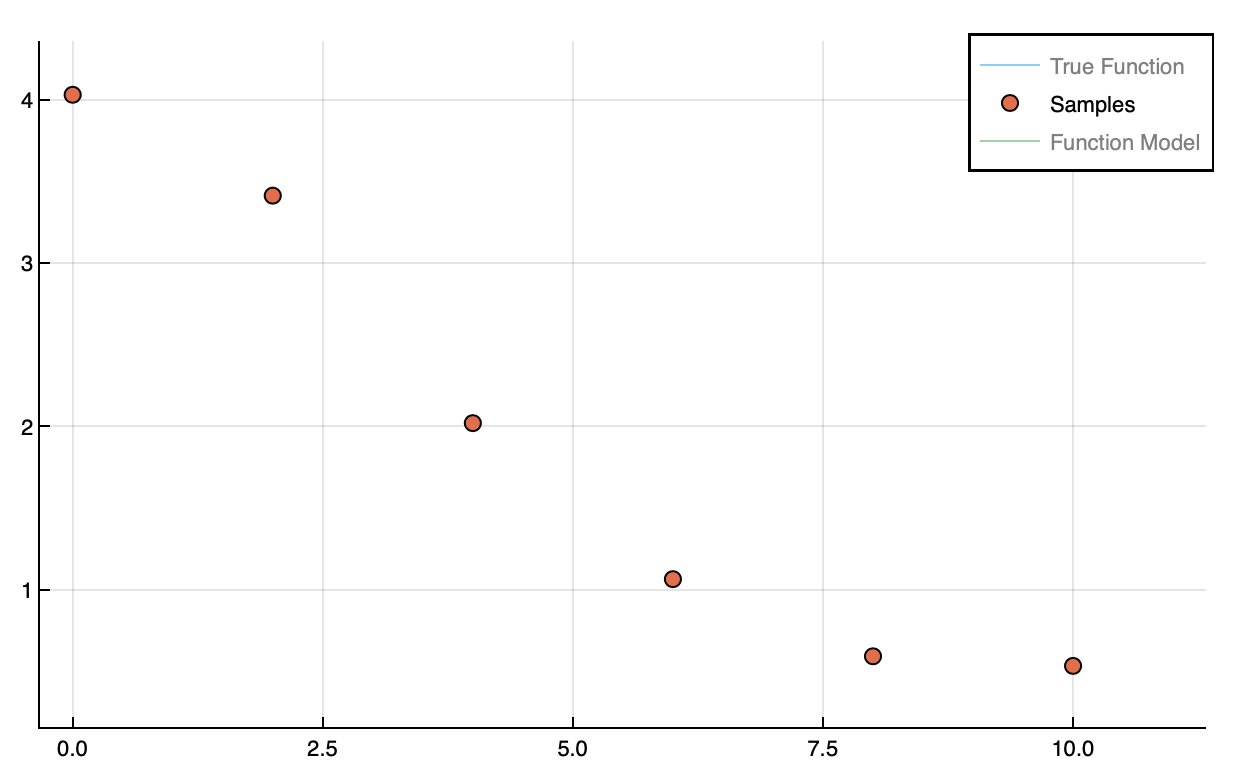
\includegraphics[scale = 0.4]{Figures/func1Samples}
\caption{An unknown function sampled by 6 data points.
\label{fig:func1Samples}} 
\end{figure}

\par Let us first make a guess of the form of the secret function. Because it looks like a simple polynomial, let us work with a power series of the form

\begin{align}
f(x) &= \sum_{n=0}^\infty b_n x^n
	\label{eq:powerSum}\\ 
&= x^0b_0 + x^1b_1 + x^2b_2 + \ldots\ .
	\label{eq:powerSeries}
\end{align}

\par The coefficients, $b_n$, will determine the shape of the polynomial.

Equation \ref{eq:powerSeries} can be evaluated at $x=2$ and written in matrix form as

\begin{equation} \label{eq:powerVectors}
\begin{bmatrix}
1 & 2 & 4 & 8 & 16
\end{bmatrix}
\begin{bmatrix}
b_0 \\
b_1 \\
b_2 \\
b_3 \\
b_4 
\end{bmatrix}
=
\begin{bmatrix}
f(2)
\end{bmatrix} .
\end{equation}

\par Equation \ref{eq:powerVectors} is the expanded form of the fundamental linear algebra equation, 

\begin{equation} \label{eq:fundLinAlg}
A\vec{b} = \vec{y},
\end{equation}
where $A$ is a matrix.

\par Evaluating Equation \ref{eq:powerSeries} at all of the data points in Figure \ref{fig:func1Samples} would increase the number of rows in the matrix. Each row in the $A$ matrix corresponds to a unique sample point.

%\par Clearly with equation (\ref{powerVectors}) we can only input one point, $(x_i,f(x_i))$, which does not provide enough information to solve for reasonable values in $\vec{b}$, the vector of coefficients. In figure \ref{figFunc1Samples} we have 6 samples, so we can repeat equation (\ref{powerVectors}) for each sample with the same coefficients. We can combine all six equations into one like so

%\par Now we can see that each row in the $x$ matrix corresponds with a row in the $f(x)$ vector. Each row represents one of our sample points, thus denoting 6 rows. This relationship between rows and individual sample points can be better visualized if subscripts are added to each respective value of $x$,

\begin{equation} \label{eq:LinAlgSubscript}
\begin{bmatrix}
1 & x_1 & x_1^2 & x_1^3 & x_1^4 \\
1 & x_2 & x_2^2 & x_2^3 & x_2^4 \\
1 & x_3 & x_3^2 & x_3^3 & x_3^4 \\
 & & \vdots & &
\end{bmatrix}
\begin{bmatrix}
b_0 \\
b_1 \\
b_2 \\
b_3 \\
b_4 
\end{bmatrix}
=
\begin{bmatrix}
f(x_1) \\ 
f(x_2) \\
f(x_3) \\ 
\vdots
\end{bmatrix}.
\end{equation}
And finally, $A$ and $\vec{y}$ can be populated with their true values,

\begin{equation} \label{eq:realValues}
\begin{bmatrix}
1 & 0 & 0^2 & 0^3 & 0^4 \\
1 & 2 & 2^2 & 2^3 & 2^4 \\
1 & 4 & 4^2 & 4^3 & 4^4 \\
1 & 6 & 6^2 & 6^3 & 6^4 \\
1 & 8 & 8^2 & 8^3 & 8^4 \\
1 & 10 & 10^2 & 10^3 & 10^4
\end{bmatrix}
\begin{bmatrix}
b_0 \\
b_1 \\
b_2 \\
b_3 \\
b_4 
\end{bmatrix}
=
\begin{bmatrix}
f(0) \\ 
f(2) \\
f(4) \\ 
f(6) \\
f(8) \\
f(10)
\end{bmatrix}
\end{equation}

\par If the $A$ matrix were square and invertible, solving for $\vec{b}$ would be as simple as $\vec{b} = A^{-1}\vec{y}$. Because there are more equations than unknowns, this is an \textit{over-determined} system; the alternative being an \textit{under-determined} system, one with more unknowns than equations.
\par There will be either no solutions, or an infinite number of solutions. In the case of infinite solutions, the solution needs to be constrained. If there are no solutions, as is often the case with an underdetermined system, a least-squares approximation can be calculated. In either case, the solutions to the linear systems become non-unique. This means there is not a single set of values for $\vec{b}$ that can solve Equation \ref{eq:fundLinAlg}.
\par In the example given, calculating one sample is quite easy, but in modeling more complicated systems, each sample becomes computationaly expensive. It will later be seen that the systems used will generally be underdetermined.
\par Solving an overdetermined system for the vector of coefficients can be done by 

\begin{align}
A\vec{b} &= \vec{y} \\
(A^TA)\vec{b} &= A^T\vec{y} \\
\vec{b} &= A^T\vec{y}, \label{eq:bSolve}
\end{align}
where $A^T$ denotes the transpose of $A$.

\par Solving an underdetermined system is done by using singular value decomposition (SVD)\cite{linAlg-book}. To solve $A\vec{b}=\vec{y}$, first find the eigenvalues and their corresponding orthonormal eigenvectors of $A^TA$. $V$ is the matrix containing these eigenvectors and $\Sigma$ contains the singular values, the square roots of each non-zero eigenvalue, on its diagonal and $0$'s elsewhere, matching the shape of matrix $A$. Each column of the matrix $U$ can be constructed by $u_k=\frac{1}{\sigma_k}A\vec{v_k}$ where $\sigma_k$ are the singular values and $\vec{v_k}$ are the columns of $V$. The final result is the complete SVD of $A$ and the solving of $\vec{b}$ from Equation \ref{eq:bSolve} by

\begin{align}
A & =U\Sigma V^T \\
\vec{b} &= (U\Sigma V^T)^T\vec{y} \\
\vec{b} &= V^{T^T}\Sigma^TU^T\vec{y} \\
\vec{b} &= V\Sigma^TU^T\vec{y}.
\end{align}

\par Now that $\vec{b}$, the vector of coefficients, has been solved for, the model can be used to predict the y position of any x value within the range of sample points. To produce a continuous visual of the model's fit, the model can take in x values for every point in the sample range and plot its respective evaluation. The result of this process can be seen in Figure \ref{fig:func1True}.

\begin{figure}[h]
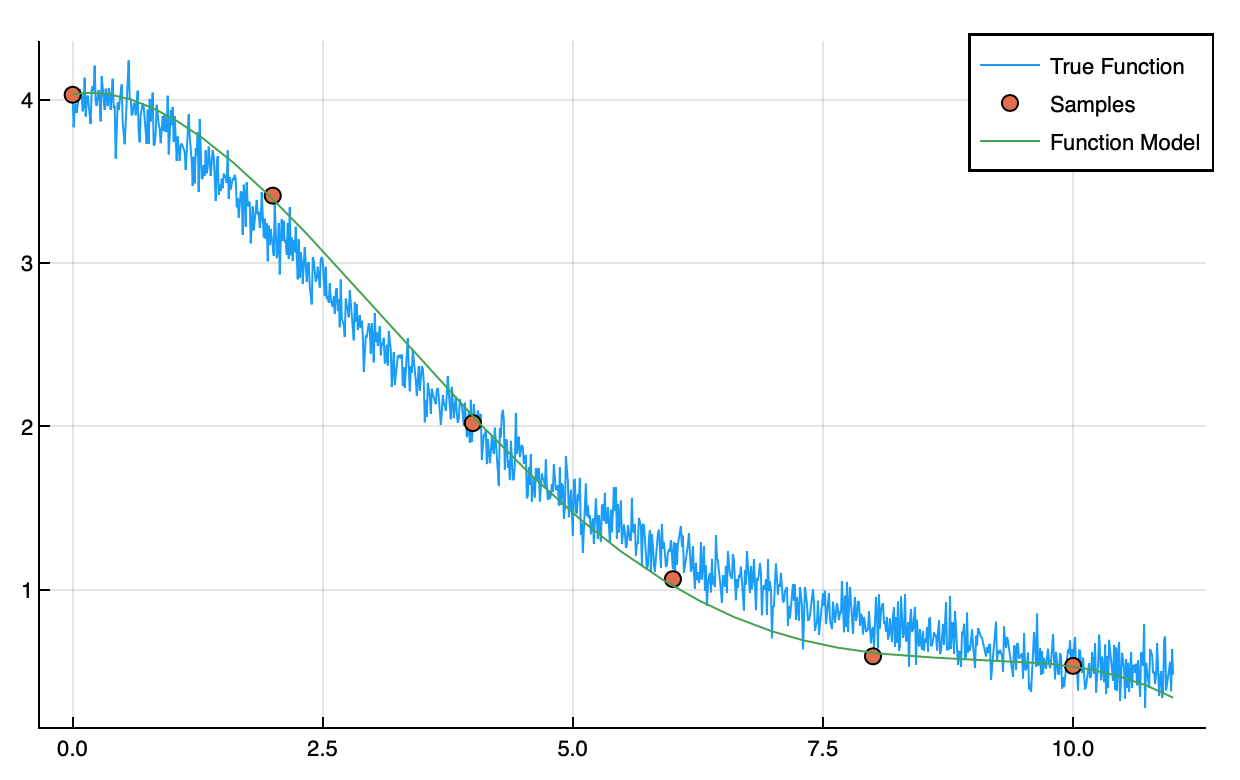
\includegraphics[scale = 0.4]{Figures/func1True}
\caption{The true function is shown by the blue line and the points are the locations of our samples. The green line shows the function created by our model to predict the true function.
\label{fig:func1True}} 
\end{figure}



\subsection{Basis Functions and Sample Size}\label{Sect:samplesAndFunctions}
\par As seen in the previous section, and in particular Equations \ref{eq:LinAlgSubscript} and \ref{eq:realValues}, each row of matrix $A$ and vector $\vec{y}$ represents a single sampling and each column is a unique basis function. It should be understood that as either of these two variables increases, thus increasing the length or width of $A$, so should the accuracy and precision of the model increase. In theory, there is no limit to the number of samples or basis vectors that could be used to construct a model, but in reality, there is a balance between the former variables and computational capabilities. In the example given, an increase in the number of samples or basis functions will not dramatically affect the computational power required, but becomes a greater concern for models of systems with increasing complexity. 
\par As discussed, the quantity of basis functions can make a large impact, but another important factor is quality. Though the choice of basis functions in the example above was simple, it can often be a difficult choice. Consider, for example, a Fourier basis. The equivalent of Equation \ref{eq:LinAlgSubscript} in this basis would be

\begin{equation} \label{eq:fourierBasis}
\begin{bmatrix}
\sin(x_1) & \sin(2x_1) \\
\sin(x_2) & \sin(2x_2) & \ldots & \ldots \\
\sin(x_3) & \sin(2x_3) \\
\vdots & & \ddots & & \\
\sin(x_n) & \ldots & & \sin(mx_n)
\end{bmatrix}
\begin{bmatrix}
b_0 \\
b_1 \\
b_2 \\
\vdots \\
b_m 
\end{bmatrix}
=
\begin{bmatrix}
f(x_1) \\ 
f(x_2) \\
f(x_3) \\ 
\vdots \\
f(x_n)
\end{bmatrix},
\end{equation}
for an $n\times m$ matrix.
\par When used in the proper circumstance, this Fourier basis can be an excellent choice for modeling a function, as in Figure \ref{fig:2dFourier}.

\begin{figure}[h]
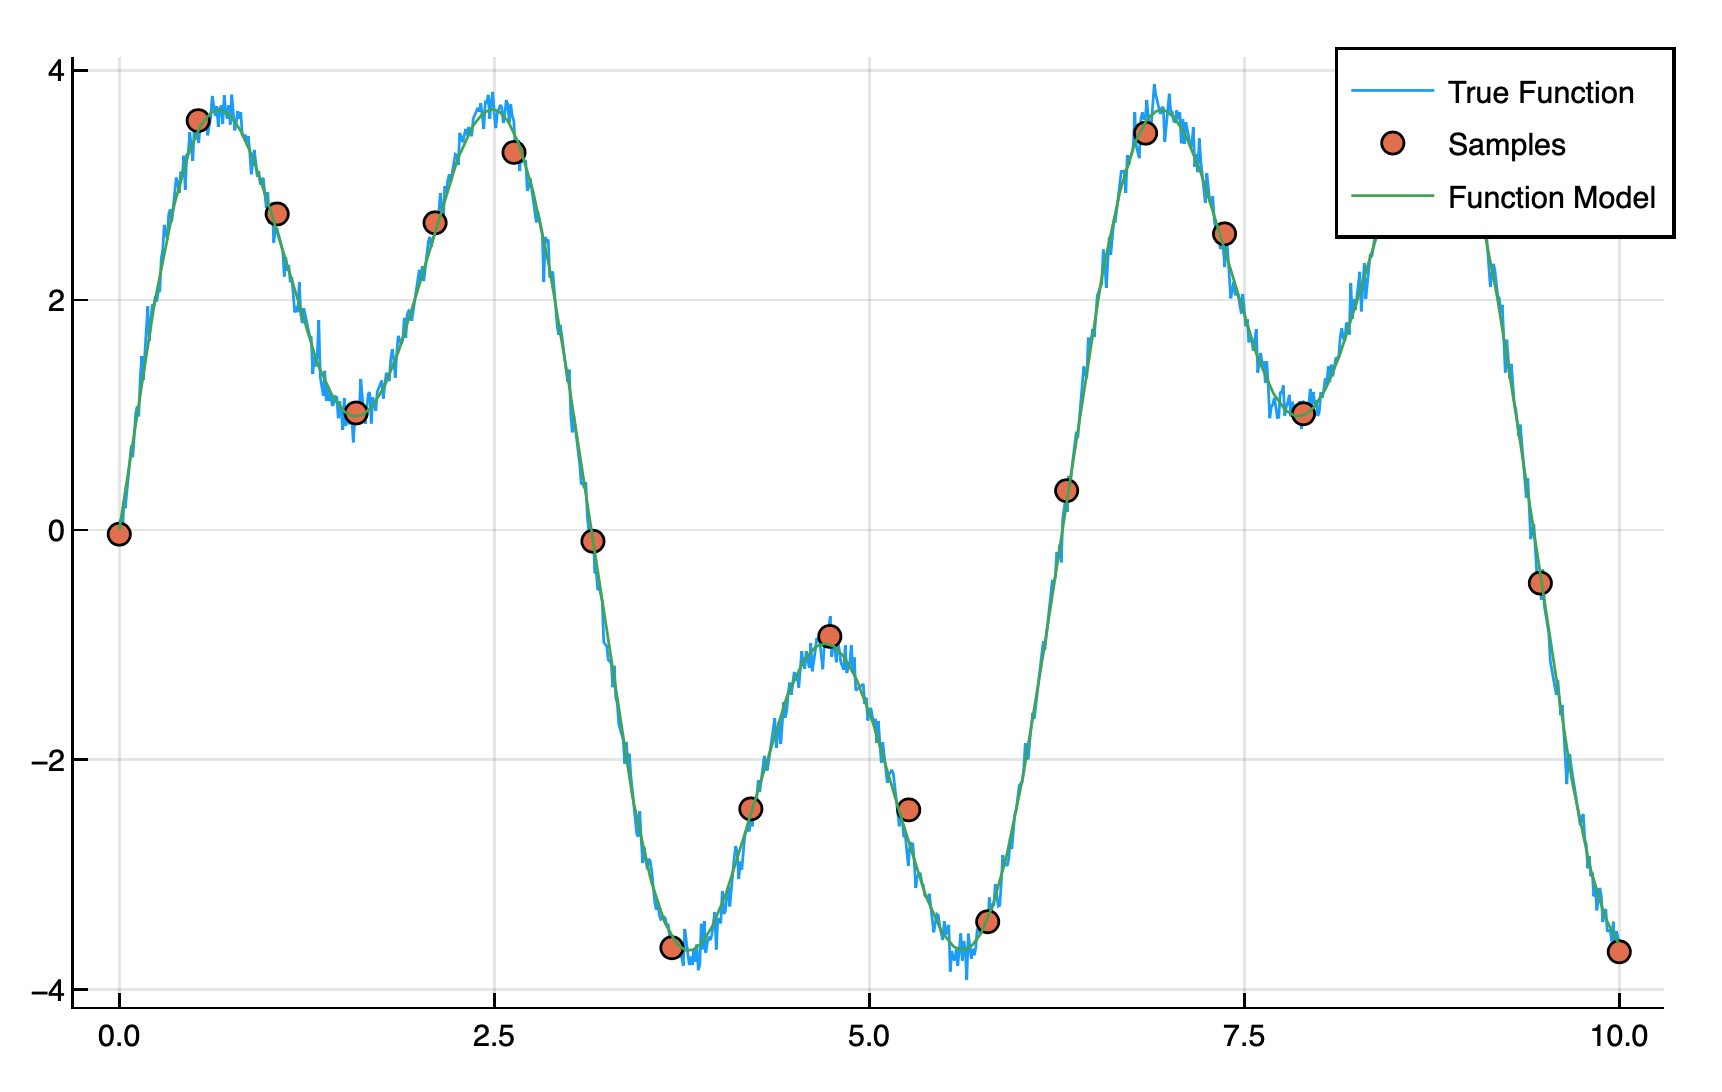
\includegraphics[scale = 0.27]{Figures/2dFourier}
\caption{The sample points shown were used to build a model of the function in green, and the true function is displayed in blue. As can be seen, a Fourier basis resulted in an excellent fit. 
\label{fig:2dFourier}} 
\end{figure}

\par When chosing sample points, there are again two things to consider: number and breadth. As will be seen later, the number of samples can have a significant impact on the time it takes to construct a model and the accuracy of said model. The breadth of samples is similarly important. If all samples from Figure \ref{fig:2dFourier} were taken between 0 and 1, the model produced would poorly estimate $f(2.5)$, as in Figure \ref{fig:poorSamps}. 

\begin{figure}[h]
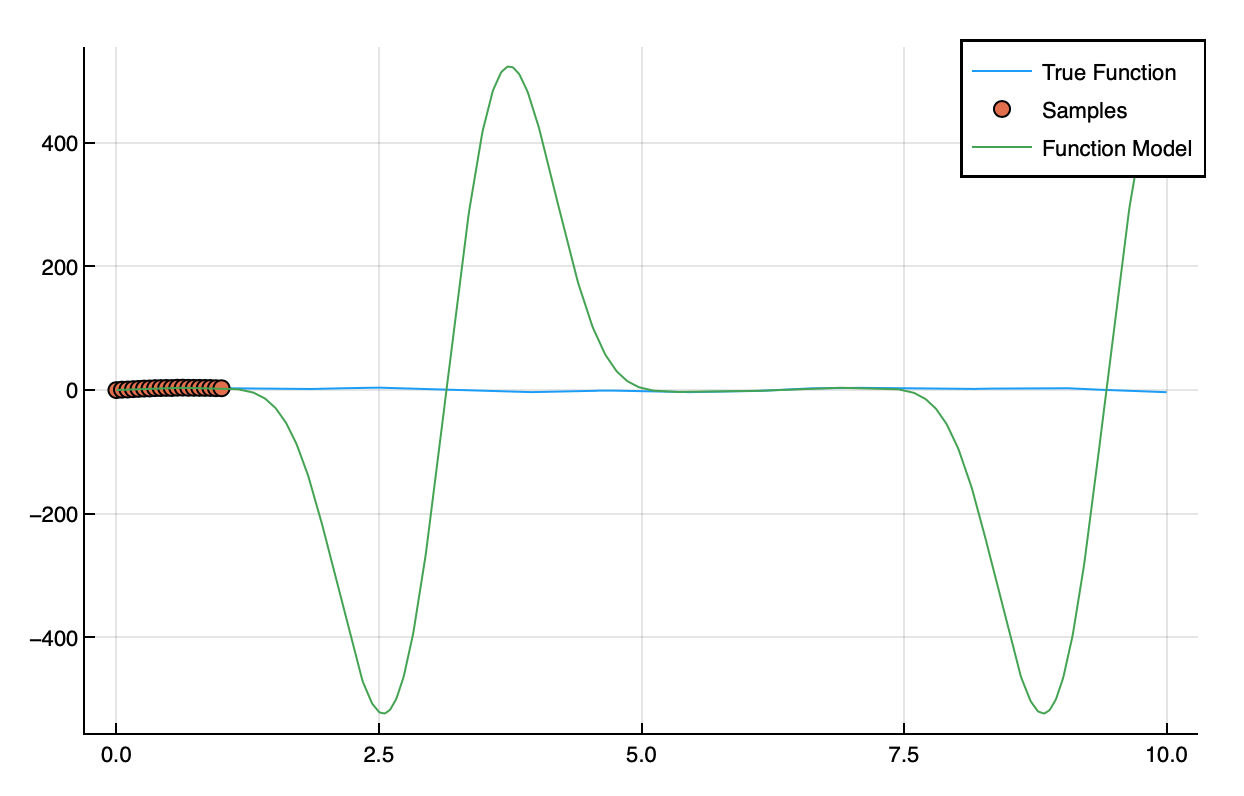
\includegraphics[scale = 0.4]{Figures/poorSamps}
\caption{A model with an insufficient breadth of samples will naturally produce a poor model. In this case, the secret function from Figure \ref{fig:2dFourier} was only sampled from the interval 0 to 1. If the model were evaluated at $x=2.5$, the fit would produce a highly inaccurate result when compared to the true function.
\label{fig:poorSamps}} 
\end{figure}

\par By this point it should be obvious to the reader that the decision of number and breadth of sample points as well as quantity and quality of basis functions is critical to the model's performance. With well chosen basis functions but poor breadth of samples, a model's accuracy can be greatly limited, as in Figure \ref{fig:poorSamps}. Figure \ref{fig:3dFourier} shows the reverse situation, good number and breadth of samples, but poorly chosen basis functions. 

%\begin{figure}[h]
%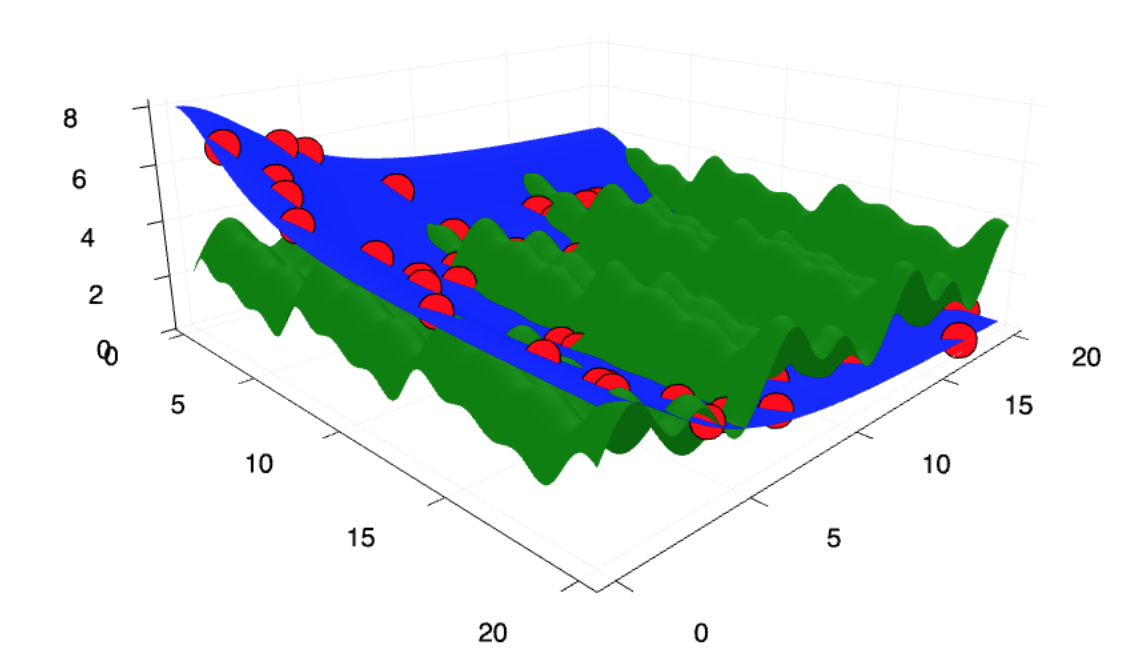
\includegraphics[scale = 0.42]{Figures/3dFourier}
%\caption{A three dimensional function in blue with a constructed model in green. The red points show the sampling of the true function. In this case, a Fourier basis is a poor choice and resulted in an inaccurate model of the true function.
%\label{3dFourier}} 
%\end{figure}

\begin{figure}
  \begin{subfigure}{0.35\textwidth}
    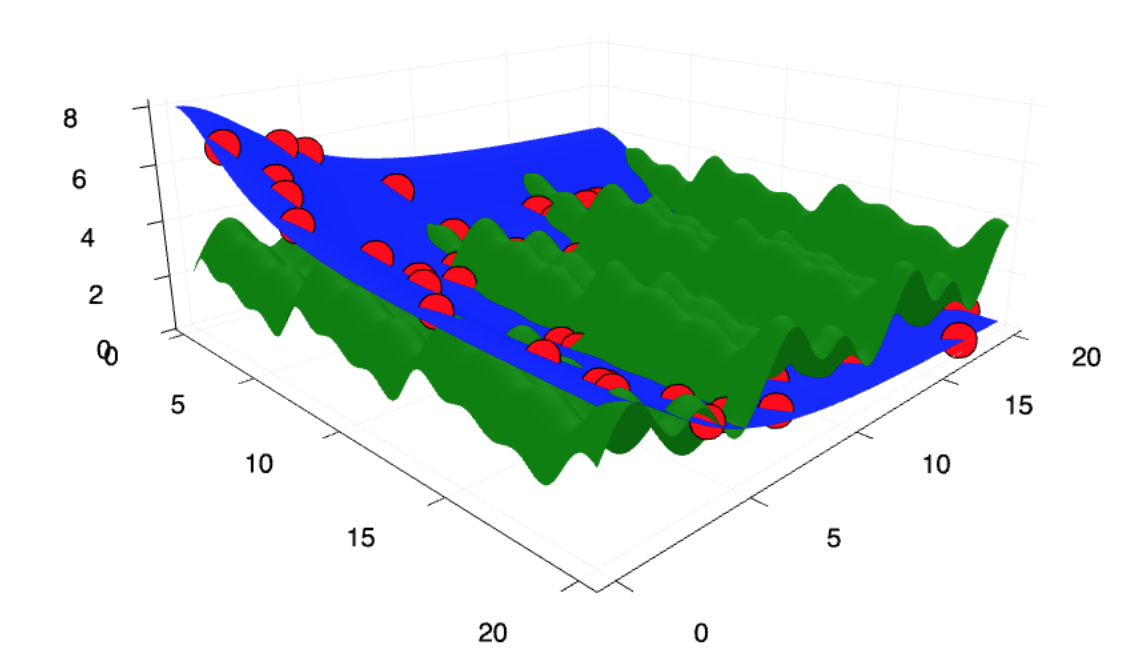
\includegraphics[width=\linewidth]{Figures/3dFourier}
    \caption{Fourier basis. $A$ is a $50\times7$ matrix.} 
    \label{fig:3dFourier}
  \end{subfigure}%
  \\
  \begin{subfigure}{0.35\textwidth}
    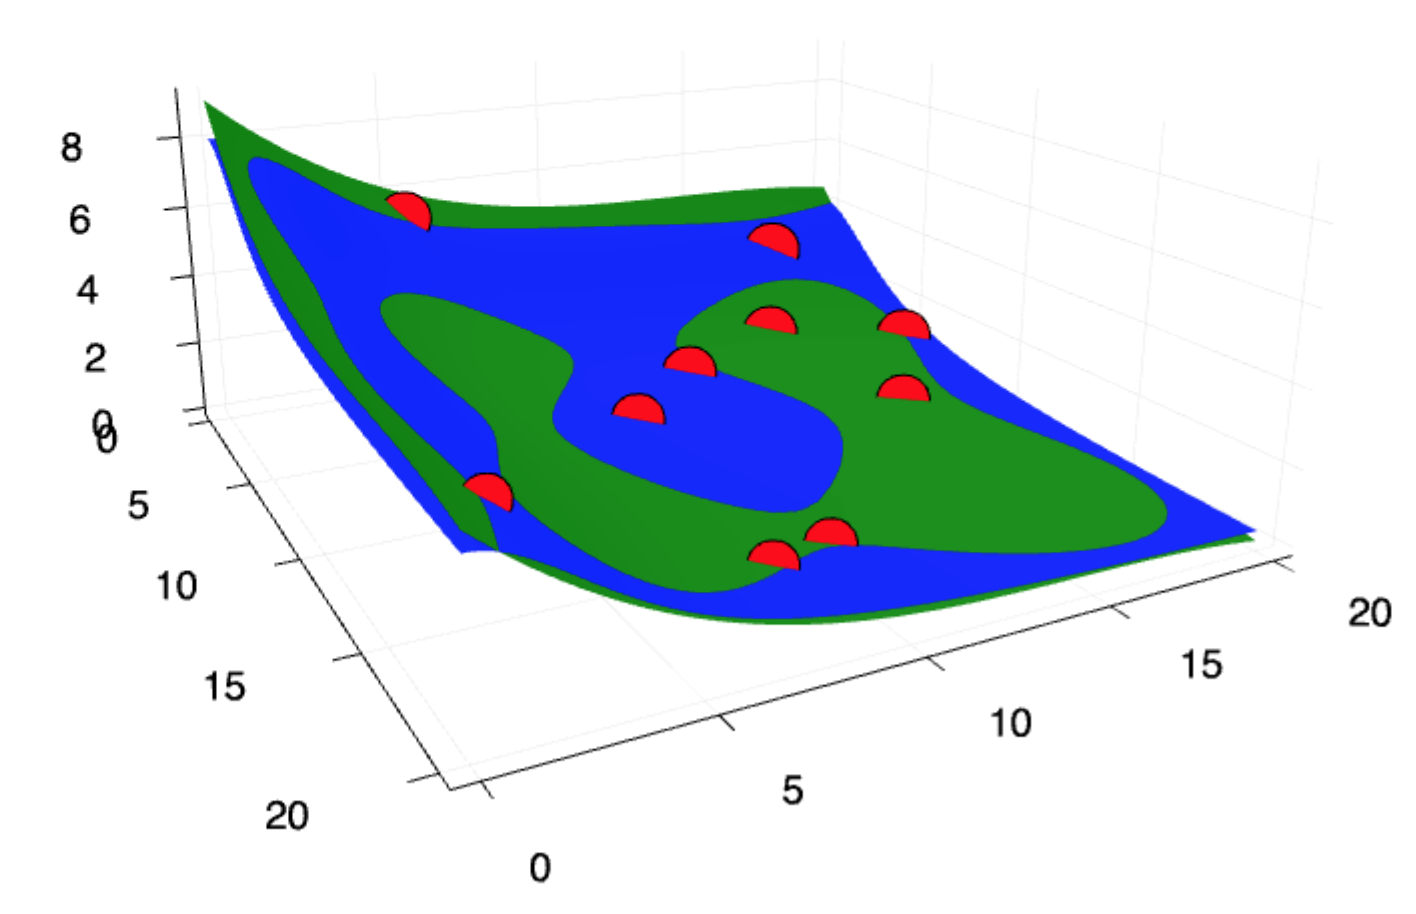
\includegraphics[width=\linewidth]{Figures/3dPower}
    \caption{Power basis. $A$ is a $10\times7$ matrix.} 
    \label{fig:3dPower}
  \end{subfigure}%
\caption{A three dimensional function in blue with a constructed model in green. The red points show the sampling of the true function. (a) In this case, a Fourier basis is a poor choice and resulted in an inaccurate model of the true function. (b) A Power series makes a convincingly better fit even with significantly fewer sample points.} \label{fig:3dFit}
\end{figure}


\subsection{Julia}\label{Sect:julia}
The figures provided throughout this paper were produced using the Julia programming language. Though encouraged to use Python for the majority of my formal education, Julia is a relatively new and fast growing language in terms of popularity. 


%Make a box figure with 10 particles
%More to be written 
\chapter{Preliminary Modeling}\label{Sect:modelPrep}

\section{Lennard-Jones Potential}\label{Sect:LJPotential}
Before jumping to the DFT data, this math and theory will be confirmed by constructing models on a simplified potential, the Lennard-Jones potential \cite{LJ-potential}. Though the Lennard-Jones potential is a simplification of reality, it does a excellent job representing real intermolecular forces of attraction and repulsion. The potential is a function of distance between two particles given by

\begin{equation} \label{eq:LJ}
V_{LJ}(r) = 4\varepsilon \bigg[\Big(\frac{\sigma}{r}\Big)^{12} - \Big(\frac{\sigma}{r}\Big)^6\bigg],
\end{equation}
where $\varepsilon$ and $\sigma$ are constants for a given particle interaction. Fig. \ref{fig:LJ} shows the plot of this potential.

\begin{figure}%[h]
\centering
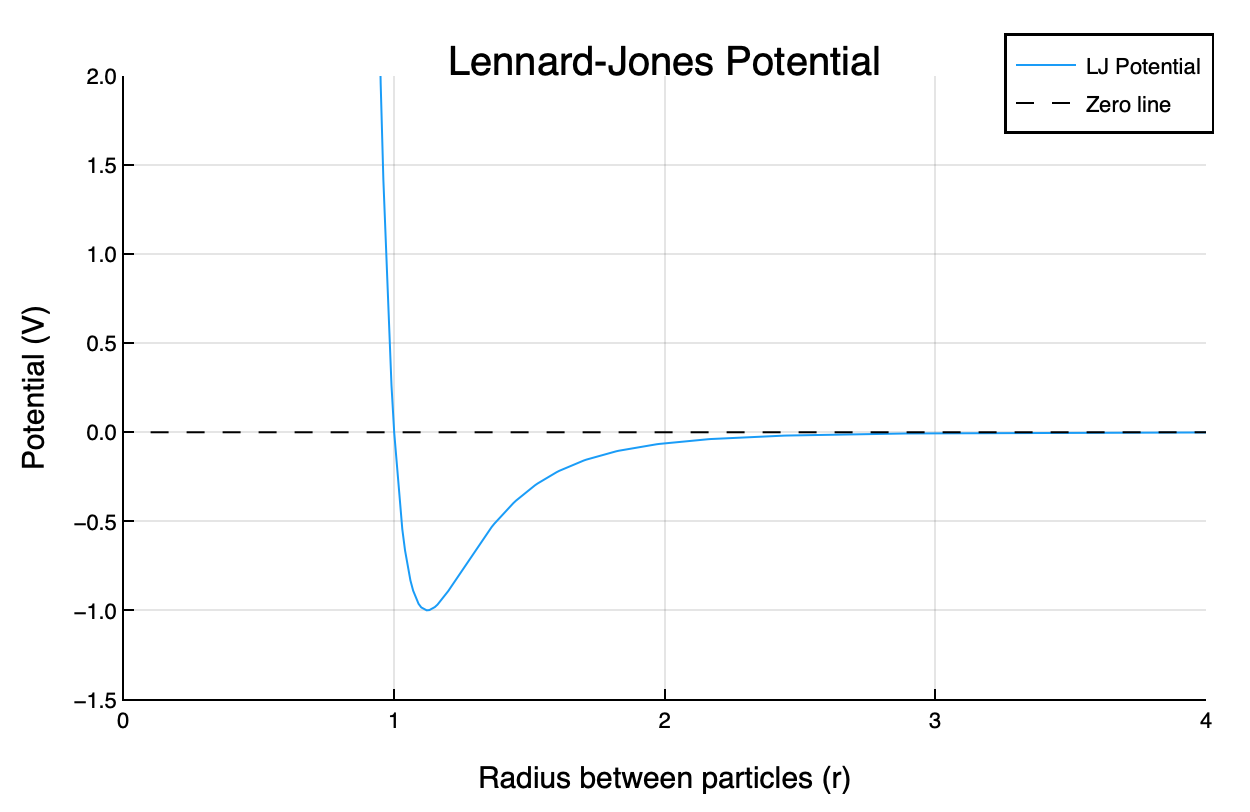
\includegraphics[scale = 0.5]{Figures/LJPotential}
\caption{The Lennard-Jones potential. A simple yet realistic model of intramolecular forces.
\label{fig:LJ}} 
\end{figure}

\par It can be recalled that the force from a potential is given by

\begin{equation} \label{eq:forceEq}
F = -\nabla U,
\end{equation}
and thus the force between two particles is zero at the bottom of the potential well. With that location as a reference, distances any greater will produce a force that is attractive and at any lesser distances, the force is intensely repulsive.
\par Calculating the potential between two particles is not difficult, but finding the total potential energy of a system of several particles becomes increasingly computationaly expensive. Because of the simplicity of the Lennard-Jones potential, the computational power required to solve for the system's energy is still relatively small. In preparation for using real, quantum-mechanical data, each system's energy will be treated as expensive to compute. 



\section{Constructing a Model}\label{Sect:LJModels}
\par Ensuring a sufficient number and breadth of samples as well as reasonable basis functions becomes difficult as the number of dimensions goes beyond 2 or 3. Ways to determine quality of samples will be discussed later and from studying a variety of potential basis functions, bessel functions of the second kind, $Y_\alpha(x)$, have potential to be useful.
\par Rewriting eq. \ref{eq:Aby} in component form yields
\begin{equation}
\begin{bmatrix}
A_{11} & A_{12} & \ldots & A_{1m} \\
A_{21} \\
\vdots & & & \vdots\\
A_{n1} & \ldots & & A_{nm}
\end{bmatrix}
\begin{bmatrix}
b_0 \\
b_1 \\
b_2 \\
\vdots \\
b_m 
\end{bmatrix}
=
\begin{bmatrix}
V_1 \\
V_2 \\
V_3 \\ 
\vdots \\
V_n
\end{bmatrix}.
\label{eq:AMatrix}
\end{equation}
\par Recognizing each row of $A$ as a unique configuration, eq. \ref{eq:AMatrix} can be written as a system of linear equations
\begin{align}
A_{11}b_1 + A_{12}b_2 + A_{13}b_3 + ... + A_{1m}b_m &= V_1 \nonumber \\
A_{21}b_1 + A_{22}b_2 + A_{23}b_3 + ... + A_{2m}b_m &= V_2 \nonumber \\
A_{n1}b_1 + A_{n2}b_2 + A_{n3}b_3 + ... + A_{nm}b_m &= V_n.
\end{align}
where $V_n$ is the total potential energy of configuration $n$. Each element of matrix $A$ will be populated as follows
\begin{align}
A_{11} &= Y_0(\alpha_{01} r_{12}) + Y_0(\alpha_{01} r_{13}) + Y_0(\alpha_{01} r_{23}) + \ldots \nonumber \\
A_{12} &= Y_0(\alpha_{02} r_{12}) + Y_0(\alpha_{02} r_{13}) + Y_0(\alpha_{02} r_{23}) + \ldots \nonumber \\
A_{1m} &= Y_0(\alpha_{0m} r_{12}) + Y_0(\alpha_{0m} r_{13}) + Y_0(\alpha_{0m} r_{23}) + \ldots \label{eq:fillBessel}
\end{align}
where $\alpha_{0m}$ is the $m$-th zero of $Y_0$, the zeroth bessel function of the first kind. Each $r_{xy}$ represents the separation vector norm ($\ell^2$ norm) for a single particle, $x$, and its pair, $y$, in the configuration. Because this model only accepts the $\ell^2$ norm of each separation vector, it is only a simple distance-dependent model using pair-interactions rather than a more complicated model using three body interactions (see Section \ref{Sect:futureWork}).

\par An example of a random assortment of particles in a box can be seen in fig. \ref{fig:tenParticles}. If two particles are generated too close together, it will cause a large spike in the system's potential. Thus a minimum separation distance must be enforced for each configuration generated. This minimum separation distance will ensure some degree of uniformity in the configurations and their total potential, effectively reducing the range of possible energies and requiring fewer training systems. 

\begin{figure}%[h]
\centering
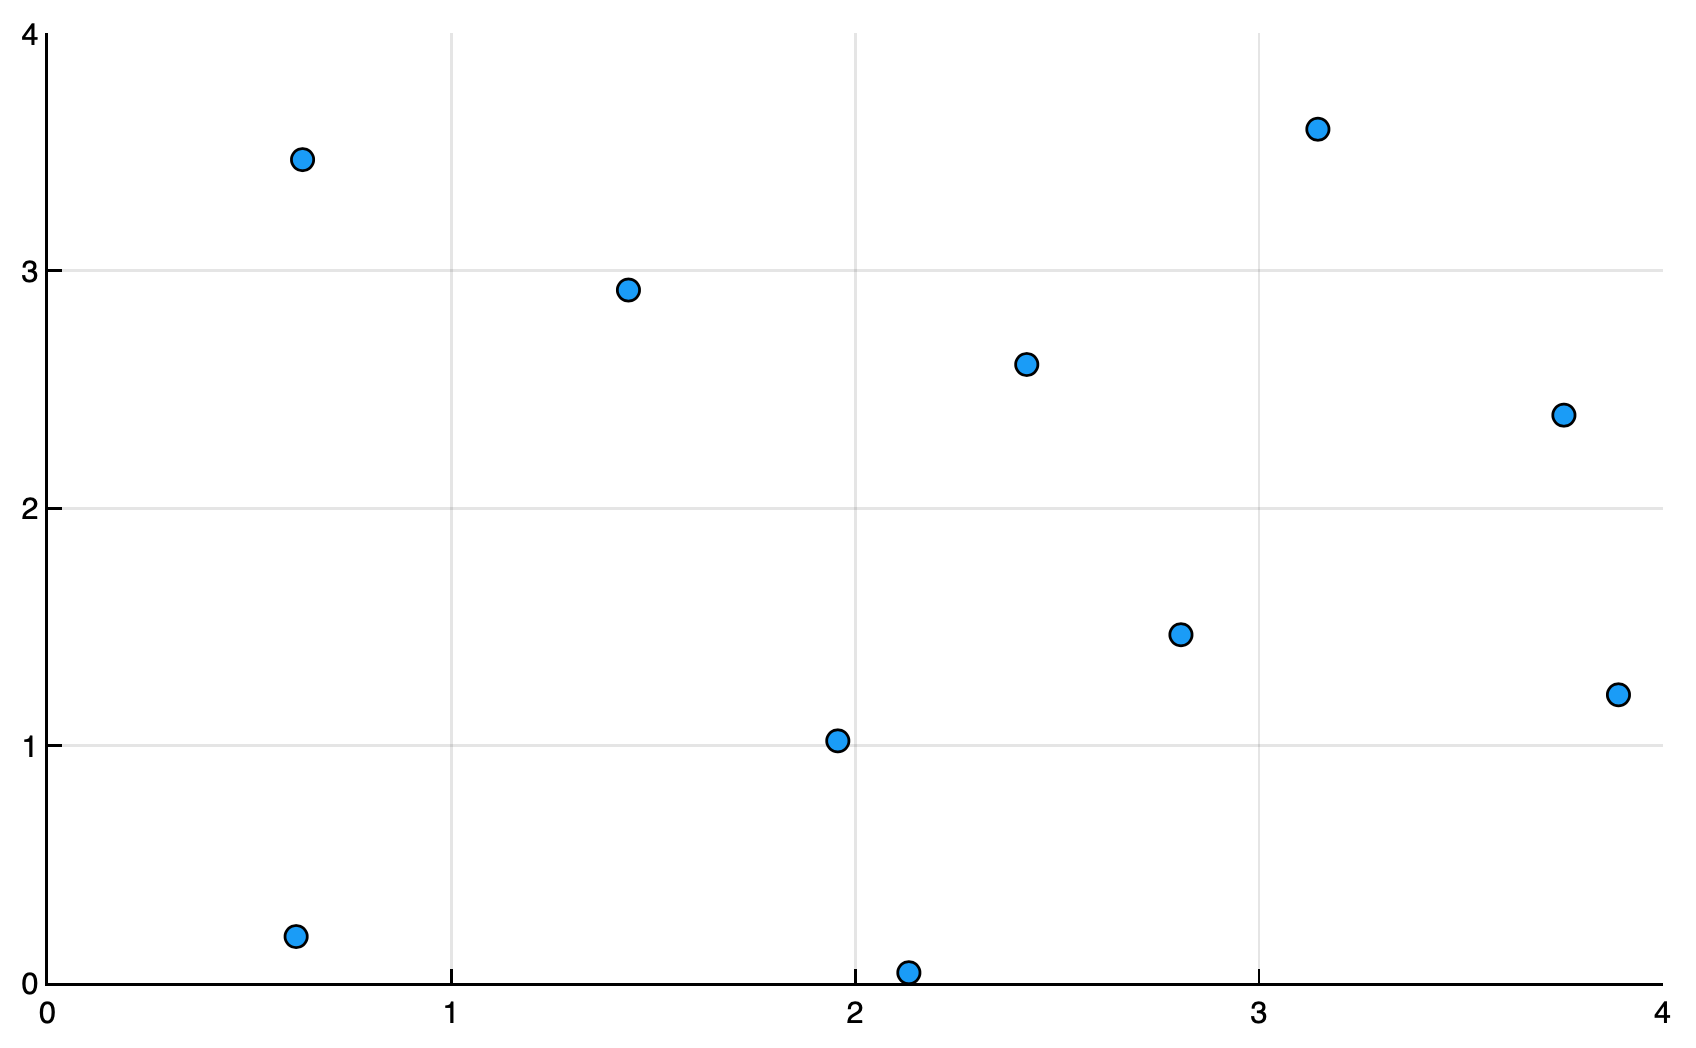
\includegraphics[scale = 0.4]{Figures/tenParticles}
\caption{A random assortment of 10 particles in a 4x4 square. No two particles are allowed to be within a pre-specified distance of each other. 
\label{fig:tenParticles}} 
\end{figure}

\par Through experimentation, the detailed relationship between size of the training set, number of basis functions, and the minimum separation distance can be outlined. In general, the accuracy of the model increases as the number of training sets and basis functions increases. The accuracy also increases when the minimum separation distance does not correspond to a particularly large potential energy. In the case of the Lennard-Jones potential in fig. \ref{fig:LJ}, the minimum separation distance has a preferred minimum of 0.8 or 0.9 to avoid large errors in the constructed model.



\section{Multi-Type Particle Systems}\label{Sect:diatomic}
\par Now that a simple monotomic model has been constructed, it can be adjusted to handle two different types of particles. The different particles can be labeled type-$A$ and type-$B$. This diatomic system will now require \textit{three} different potential equations, one describing each type of interaction. The three unique interactions are type-$A$ interacting with another type-$A$, a type-$A$ interacting with a type-$B$, and a type-$B$ with another type-$B$. Because these are arbitrary interactions (due to unspecified atomic structure), they can be defined by choosing reasonable values of $\varepsilon$ and $\sigma$ from eq. \ref{eq:LJ}. 
\begin{align}
V_{AB}(r) &= 4 \bigg[\Big(\frac{1}{r}\Big)^{12} - \Big(\frac{1}{r}\Big)^6\bigg] \label{LJ} \\
V_{AA}(r) &= 4 (0.7) \bigg[\Big(\frac{0.8}{r}\Big)^{12} - \Big(\frac{0.8}{r}\Big)^6\bigg] \label{LJ} \\
V_{BB}(r) &= 4 (0.4) \bigg[\Big(\frac{1.1}{r}\Big)^{12} - \Big(\frac{1.1}{r}\Big)^6\bigg] \label{LJ}
\end{align}
The graph of each potential can be seen in fig. \ref{fig:3LJ}. Each of the equilibrium positions and energies is slightly different, but all in the same neighborhood.

\begin{figure}%[h]
\centering
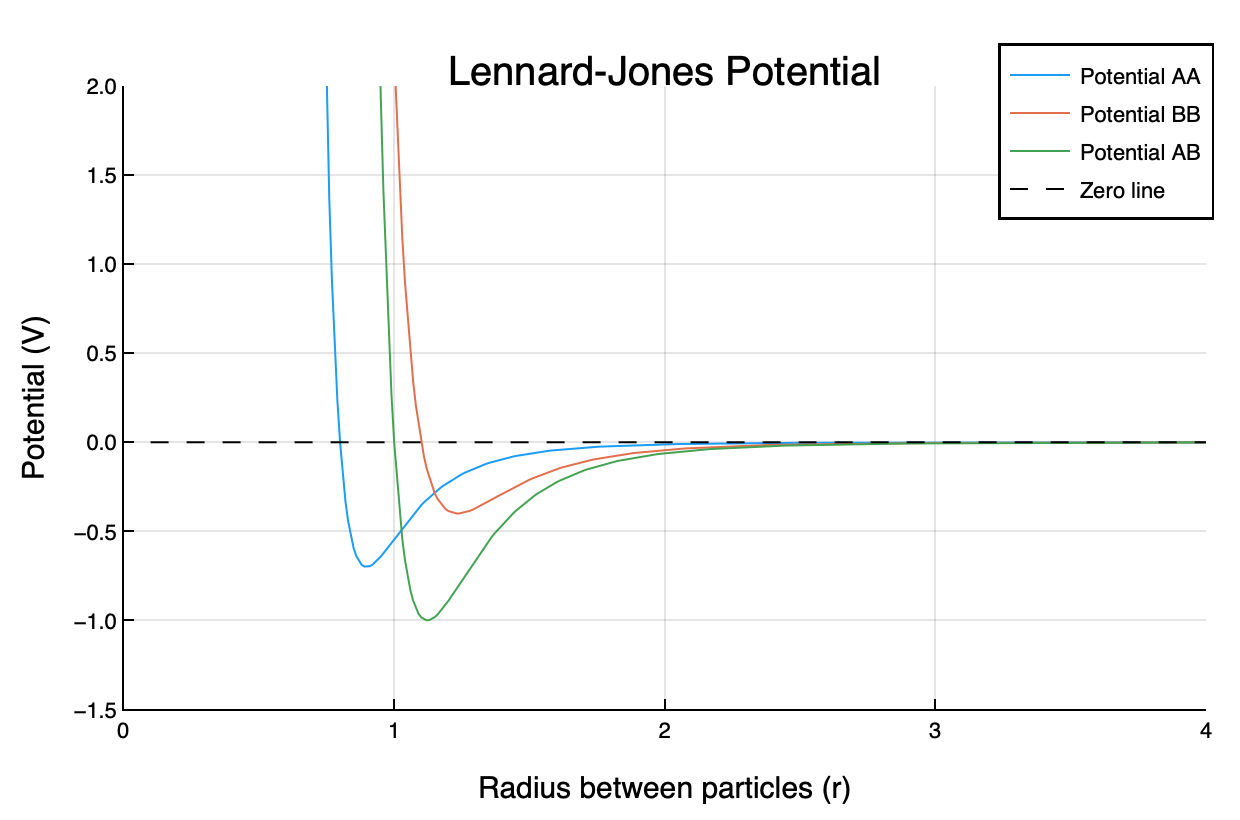
\includegraphics[scale = 0.5]{Figures/newLJPotential}
\caption{A Lennard-Jones potential for each particle interaction type (AA, AB, and BB). Each interaction potential has a slightly different equilibrium position and energy. 
\label{fig:3LJ}} 
\end{figure}

\par To handle this increase in complexity, matrix $A$ will need to contain \textit{three} columns where the previous model had only one. This is also because of the three different interaction types, one column for each. Another obstacle arises in the decision for particle type ratio. If the particle number (10) and box size ($4\times4$) remain constant, how many type-$A$ versus type-$B$ particles should there be to help train an effective model?
\par This question can be generalized to ask: what is a sufficient breadth of samples for this model? The answer depends greatly upon the desired range of predictions. As will be seen in Section \ref{Sect:procedureData}, the actual configurations vary in particle number and particle type ratio. Therefore, the model constructed here should be trained and tested using a spread of values for those two variables. Each training and testing set will thus be populated by a random number and ratio of particles. 
\par Once a model has been properly constructed and trained, its accuracy can be visually determined by plotting each system's predicted energy versus its actual energy. An example of this type of plot can be seen in fig. \ref{fig:diatomicAccuracy} and will be used again later on.

\begin{figure}%[h]
\centering
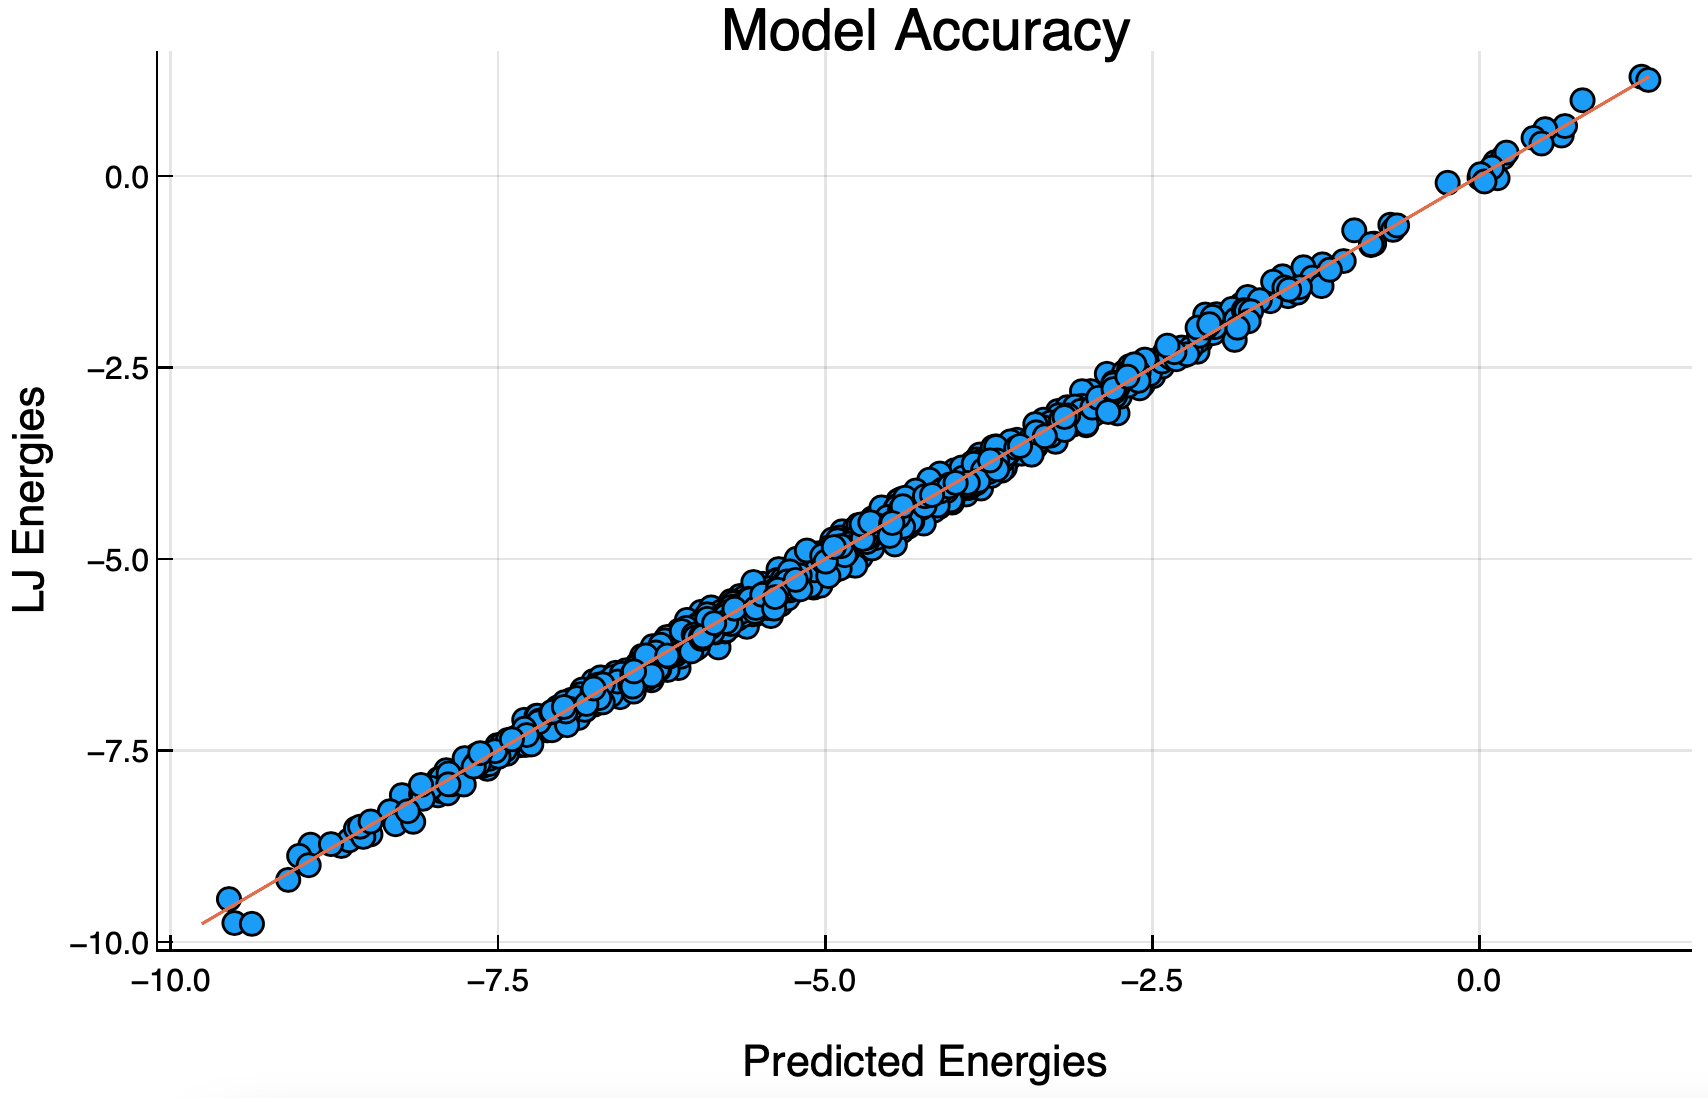
\includegraphics[scale = 0.4]{Figures/diatomicAccuracy}
\caption{1000 tests of a model with a training size of 300 systems, 900 total basis functions, and a spread of particle type ratios each for a 10 particle system. The fit is very good, denoting a highly accurate model.
\label{fig:diatomicAccuracy}}
\end{figure}

\par Now that a successful model has been created for a simplified potential, it can be adapted to fit real data in the hopes of producing useful data faster than current models.
 
\section{Procedure} \label{Sect:procedure}
\subsection{Quantum Mechanical Data}\label{Sect:procedureData}
\par First-principles calculations were performed within the framework of AFLOW\cite{} which employs the VASP software for computing energies.\cite{} Projector-augmented-wave (PAW) potentials were used and exchange-correlation functionals parametrized by Perdew, Burke, and Ernzerhof under the generalized gradient approximation (GGA)\cite{}. A dense $k$-mesh scheme was used to perform the numeric integration over the Brillioun zone\cite{}. Optimal choices of the unit cells, by standardization of the reciprocal lattice, were adopted to accelerate the convergence of the calculations.
\par As previously discussed, the process of obtaining this data was computationally expensive, creating a bottleneck in the discovery of novelty alloys. The culmination of this research is to produce a simpler model that can be trained on the given data to reproduce expected configuration energies within a range of reasonable error. Figure \ref{histEnergy} shows a histogram of all the configuration energies in the data set.

\begin{figure}[h]
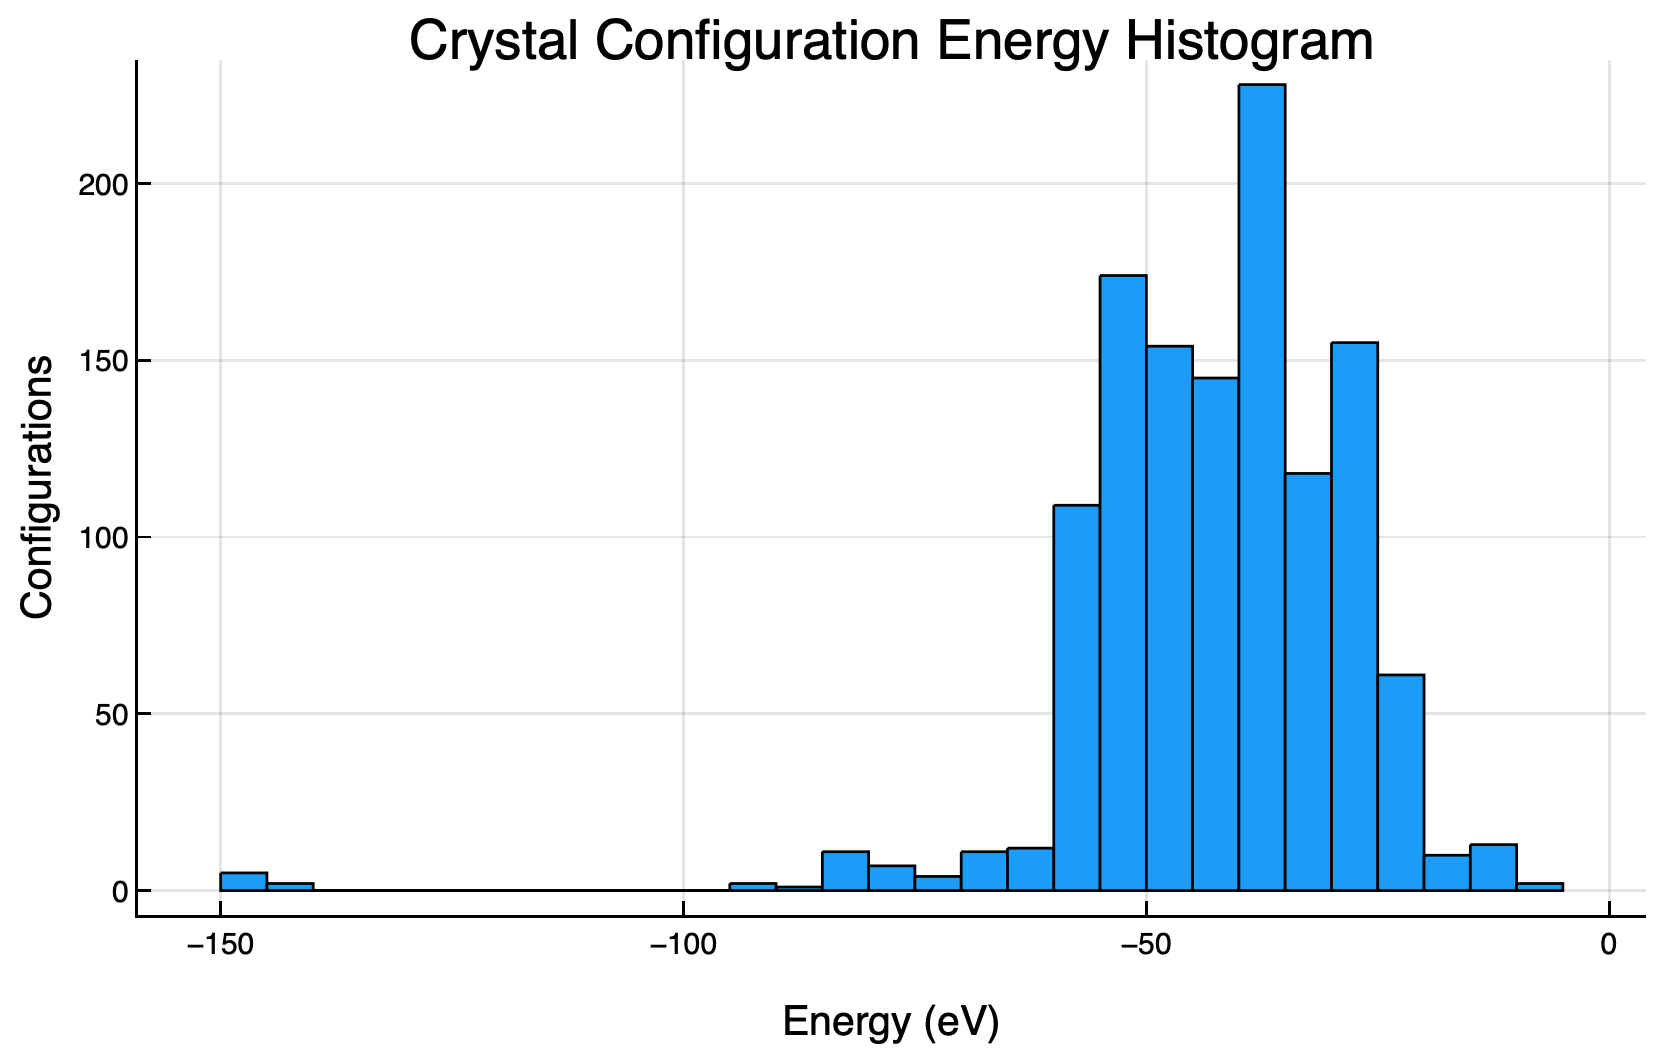
\includegraphics[scale = 0.3]{Figures/UnitCellEnergies}
\caption{A histogram showing all the configuration energies in the original data file. The majority lie within the $-20$eV to $-60$eV range, with a few outliers around $-150$eV.
\label{histEnergy}} 
\end{figure}

\par Each configuration in the data represents a unique primitive unit cell. A unit cell is the building block of any crystal structure. Each unit cell is an identical copy of every other, with the same shape, size, and contents. A \textit{primitive} unit cell is the smallest possible unit cell which contains only one of each uniquely positioned atoms in the crystal\cite{solidStateBook}. An example of a primitive unit cell configuration can be seen in Figure \ref{primitiveUnitCells}.

\begin{figure}
  \begin{subfigure}{0.25\textwidth}
    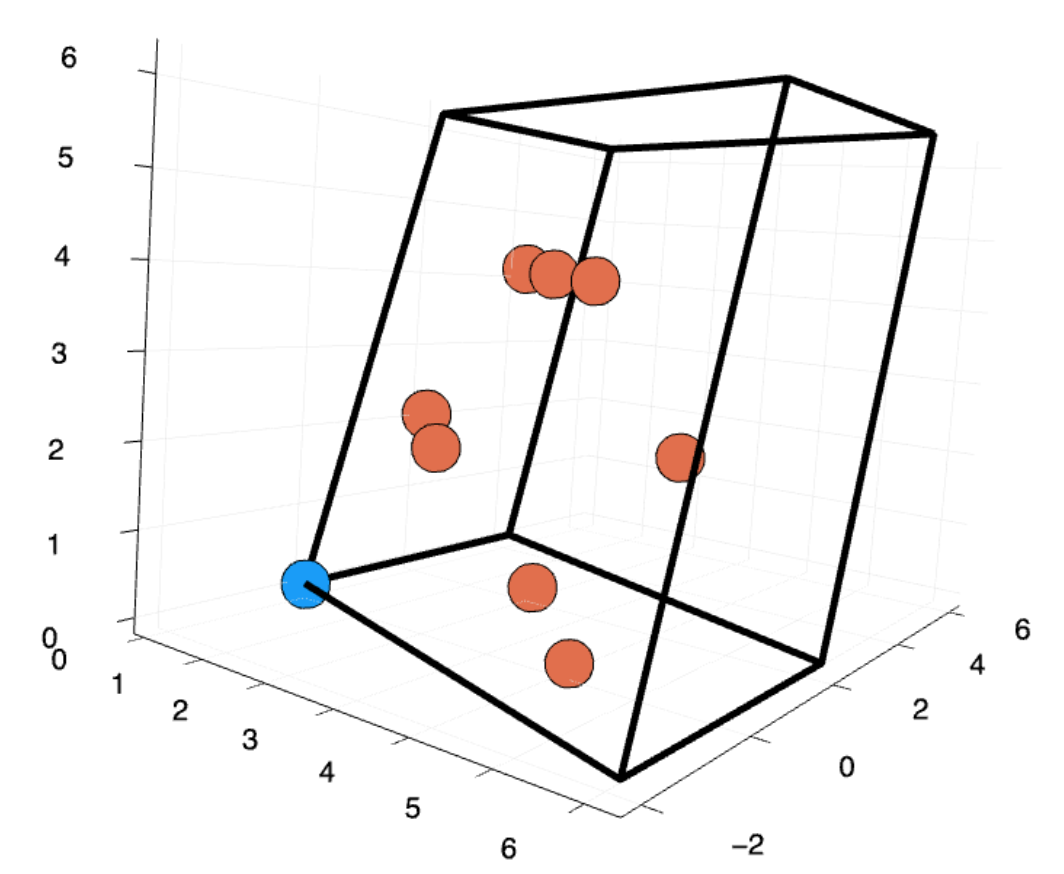
\includegraphics[width=\linewidth]{Figures/primitiveCell1}
    %\caption{First subfigure} 
    \label{primitiveFirst}
  \end{subfigure}%
  \hspace*{\fill}   % maximize separation between the subfigures
  \begin{subfigure}{0.23\textwidth}
    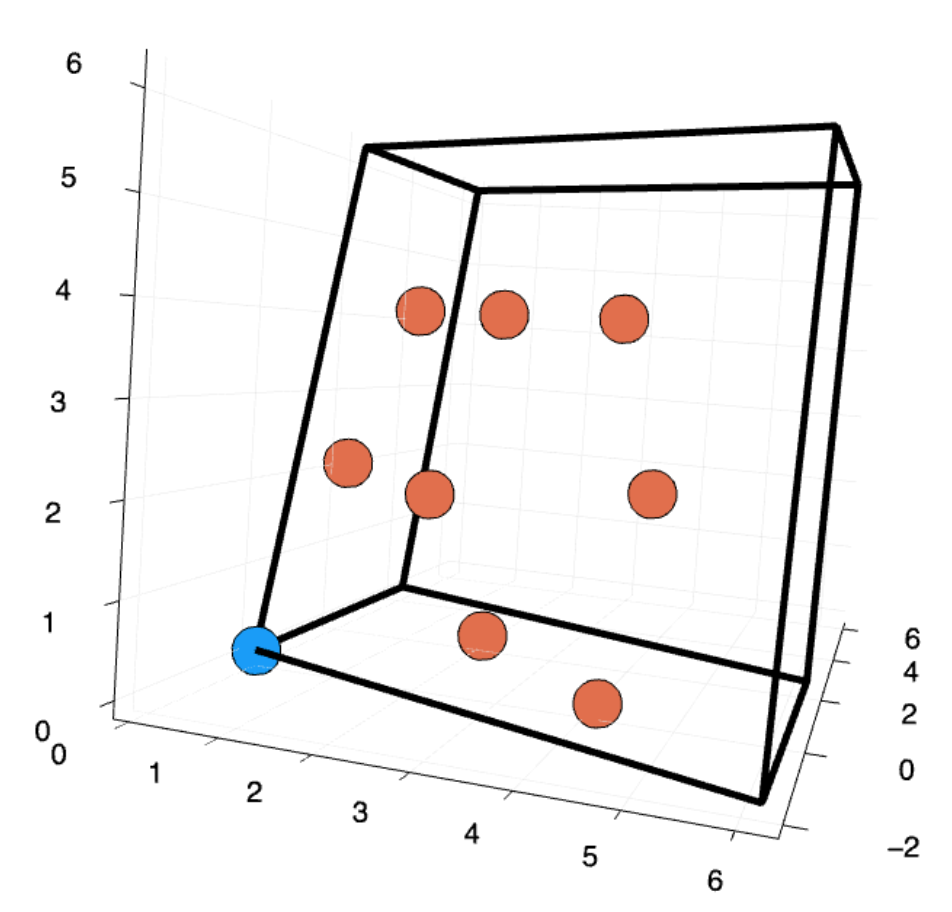
\includegraphics[width=\linewidth]{Figures/primitiveCell2}
    %\caption{Second subfigure} 
    \label{primitiveSecond}
  \end{subfigure}%
\caption{The primitive unit cell for configuration 65 from two different perspectives. The blue point is the single Ag atom while each red point shows each Pt atom in said configuration.} \label{primitiveUnitCells}
\end{figure}

\par To use the data in the \textit{.txt} file, it needs to be parsed into vectors that can be easily manipulated. An example of the data being parsed can be seen in Figure \ref{system2data}. The number on the second line is the lattice parameter, followed by three lattice vectors in $(i,j,k)$ coordinates. The line following contains two numbers, the first is the number of silver (Ag) atoms in the unit cell and the second is the number of platinum (Pt) atoms. In direct coordinates (in terms of the lattice vectors) the positions of each silver and platinum atom are then given. The last line in this system tells the total potential energy of the unit cell configuration. 

\begin{figure}[h]
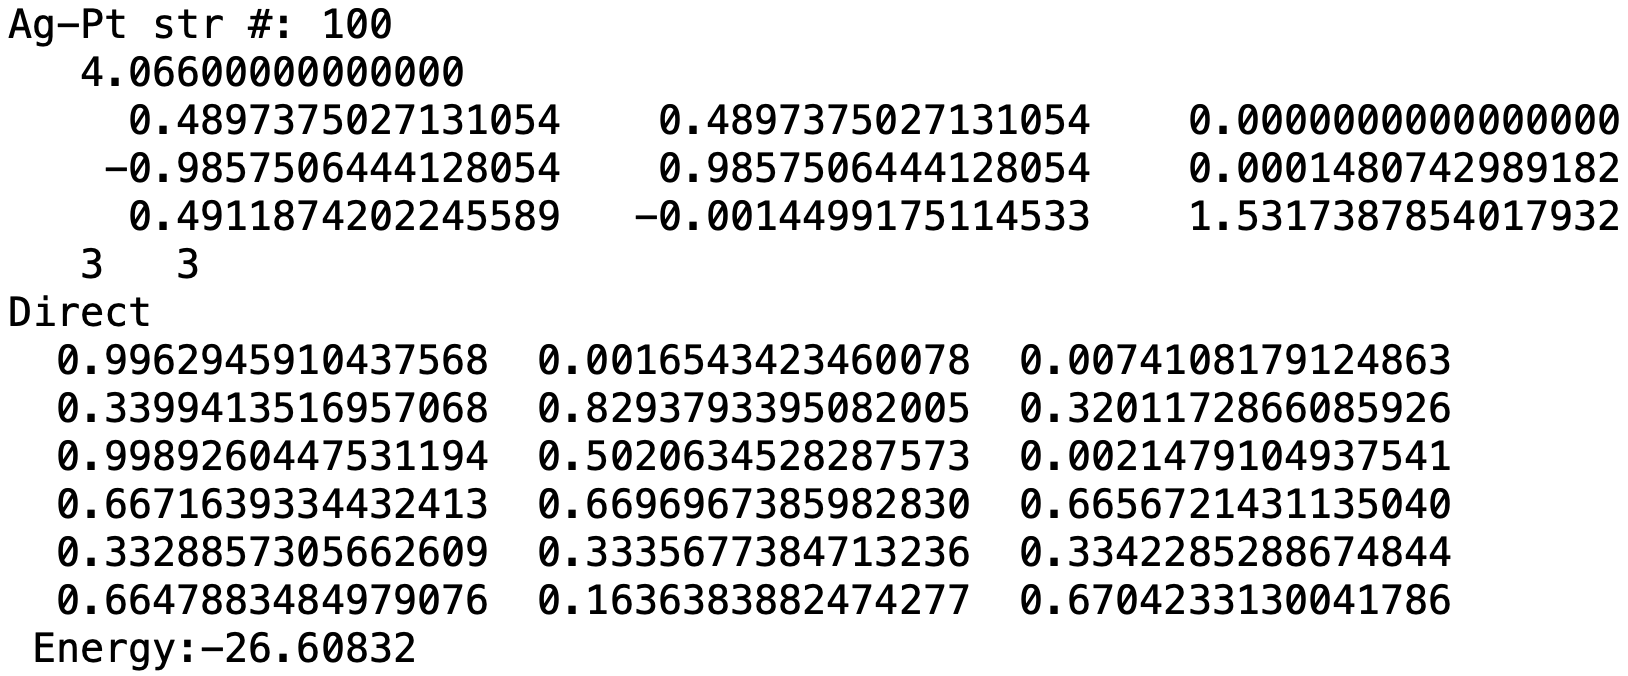
\includegraphics[scale = 0.3]{Figures/system2}
\caption{An example of the data given in AgPtdata.txt that needs to be used to build the model.
\label{system2data}} 
\end{figure}

\subsection{Model Construction}\label{Sect:procedureConstruction}
\par With the file parsed and the important data retrieved, the process of building a model can commence. The potential energy of a single particle is due to its interactions with all its surrounding particles, thus to account for each interaction with nearby particles the unit cell must be propagated outwards in all three dimensions. All atomic pairs can be enumerated by adding multiples of the lattice vectors. Then the relative position of each affecting particle can be determined and the vector separating the particle pair can be calculated. These separation vectors are the information that will be passed into the basis function to construct the model. 
\par Because the affect two particles have on each other drops off as a function of distance (similar to the Lennard-Jones potential), the unit cell does not need to be propogated infinitely in each direction, only out to a radius of reasonable influence, creating an imaginary sphere beyond which all interactions are negligible. It should be clear that the choice of this radius will make a significant impact on the quality of the model. It should also be noted that one arbitrarily chosen radius cannot be applied effectively to each unique system. A simple solution is to make the radius of this sphere of influence equal to the magnitude of the largest lattice vector multiplied by a constant. The effect of this constant on the model's precision can be tested later, but for now will be chosen to be 1.2.
\par The simplification of reality due to this ``sphere of influence" gives a clear upper bound to our unit cell propagation. It is expected that the unit cell will be propagated out further than the radius in each direction, thus encapsulating said sphere. An example of this iterated unit cell can be seen in Figure \ref{iteratedUnitCells}. 

\begin{figure}
  \begin{subfigure}{0.47\textwidth}
    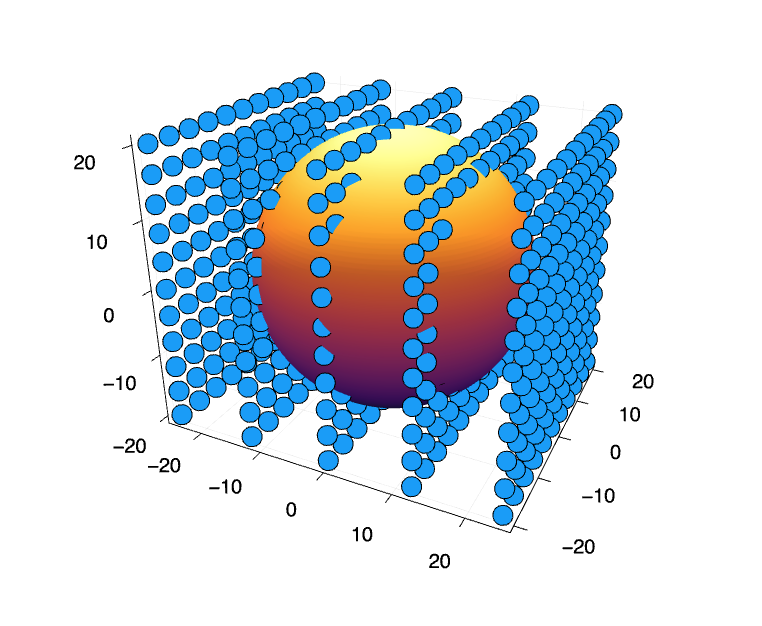
\includegraphics[width=\linewidth]{Figures/iteratedUnitCell}
    %\caption{First subfigure} 
    \label{iteratedUnitCellFirst}
  \end{subfigure}%
  \\
  %\hspace*{\fill}   % maximize separation between the subfigures
  \begin{subfigure}{0.45\textwidth}
    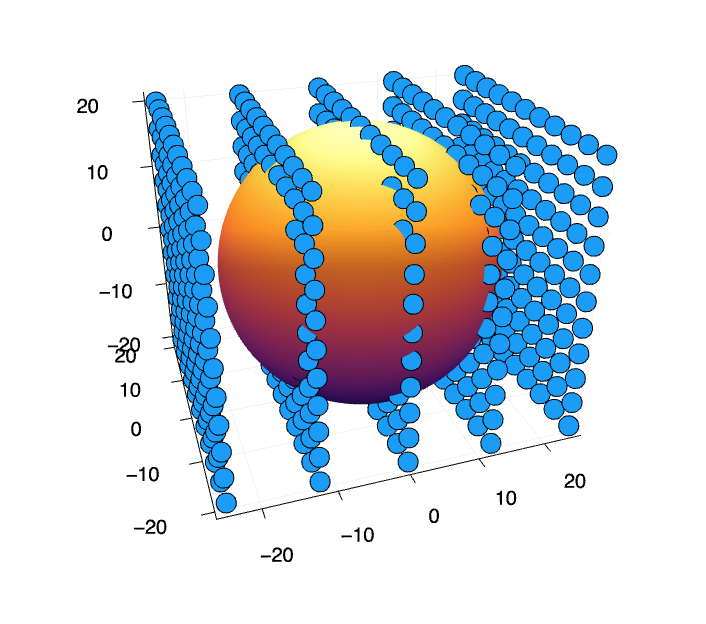
\includegraphics[width=\linewidth]{Figures/iteratedUnitCell2}
    %\caption{Second subfigure} 
    \label{iteratedUnitCellSecond}
  \end{subfigure}
\caption{The sphere of influence for one silver atom is completely encapsulated by the unit cell's iterations from two different perspectives. Only one particle from each unit cell is shown.} \label{iteratedUnitCells}
\end{figure}

Each unit cell in Figure \ref{iteratedUnitCells} can now be populated with all the contained atoms. Every atom inside the sphere can then be extracted. When these atoms are stored into a new vector, they can be plotted as in Figure \ref{plotAgAtomSphere}. When this process is repeated for every system in the DFT data, the result is a vector containing these ``important positions" for each unique silver and platinum atom in each unit cell. The separation vector norms can be quickly calculated and stored.

\begin{figure}[h]
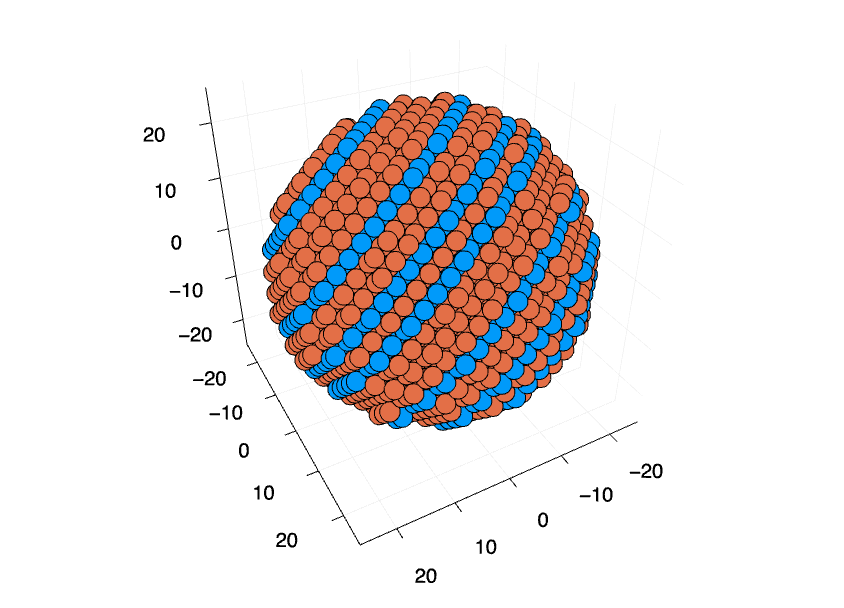
\includegraphics[scale = 0.6]{Figures/plotAgAtomSphere(3,1)}
\caption{Every silver and platinum atom inside the sphere of interest. According to the model, these are the only atoms interacting with the central atom in question. This data is taken from the first silver atom in the third sample system. 
\label{plotAgAtomSphere}} 
\end{figure}

With all the pertinent information from the data organized into vectors, construction of the $\mathbf{A}$ matrix can begin. As in the Lennard-Jones example, each row represents a crystal structure and each column corresponds to a unique basis function. And as explained in Section \ref{Sect:diatomic}, a single basis function will result in three columns of $\mathbf{A}$ due to each type of interaction. The method of populating $\mathbf{A}$ will be the same as was done earlier in Equation \ref{eq:fillBessel}. With 300 basis functions, the first 300 columns of $\mathbf{A}$ will be calculated using the separation vector norms from Ag-Ag interactions. The following 300 columns from Pt-Pt interactions and the final 300 from Ag-Pt.
\par The size of the training set is limited to 1224, the number of systems given in the data set. Whatever systems are not included in the training set will comprise the holdout set, used for testing the model's accuracy.
%\par The basis functions will again be chosen to be bessel functions of the second kind. This is because of the similarity in potential energy between two atoms as a function of distance and the shape of the graph of said bessel functions. 
\par Once the model is fully constructed, tests can be run to determine the effect of radius, sample number, and number of basis functions on the precision and accuracy of the model. An increase of radius, sample number, or number of basis functions will make significant impacts on the program runtime. As the radius is increased, the unit cell must be propagated out further to encapsulate the sphere of influence and more atom interactions will be considered. For every basis function added, there will be three columns added to the $\mathbf{A}$ matrix, drawing out its construction times. 
\par Generally, as the number of basis functions is increased and the radius of influence extended, the model's predictions will become increasingly reliable. On the other hand, as those factors increase accuracy and precision, they also increase the computational costs. It would be ideal to find a manageable trade off between the program's runtime and reliability. To investigate the quality of the model as a function of cutoff radius, sample number, and number of basis functions, a sweep can be conducted over a range of values for each and the details of the fit for each combination can be recorded. Rather than run this script on an ordinary desktop computer, it was completed on Mary Lou, BYU's supercomputer. 


\section{Results and Analysis}\label{Sect:results}
\par Introduction lines... Test
\par The quality of a single fit is given in Figure \ref{outputExample}. For some models, there are predictions that differ significantly, more than 100eV, from their true values. In those cases, the number of outlying crystals has been counted then excluded from the average error calculation. In this way, the average error can become independent of the model's outliers. To understand a given model's accuracy and precision visually, each prediction energy can be plotted against the actual energy for each configuration. The model referenced in Figure \ref{outputExample} can be seen again in Figure \ref{accuracyPlot}.

\begin{figure}[h]
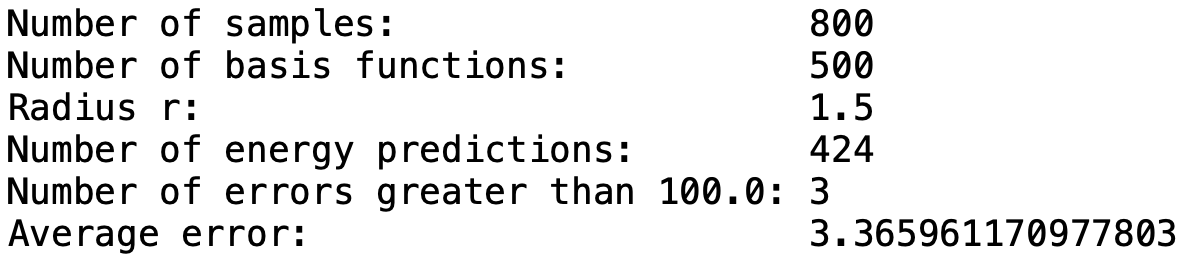
\includegraphics[scale = 0.4]{Figures/outputExample}
\caption{An example of the data in the output file. 
\label{outputExample}} 
\end{figure}

\begin{figure}[h]
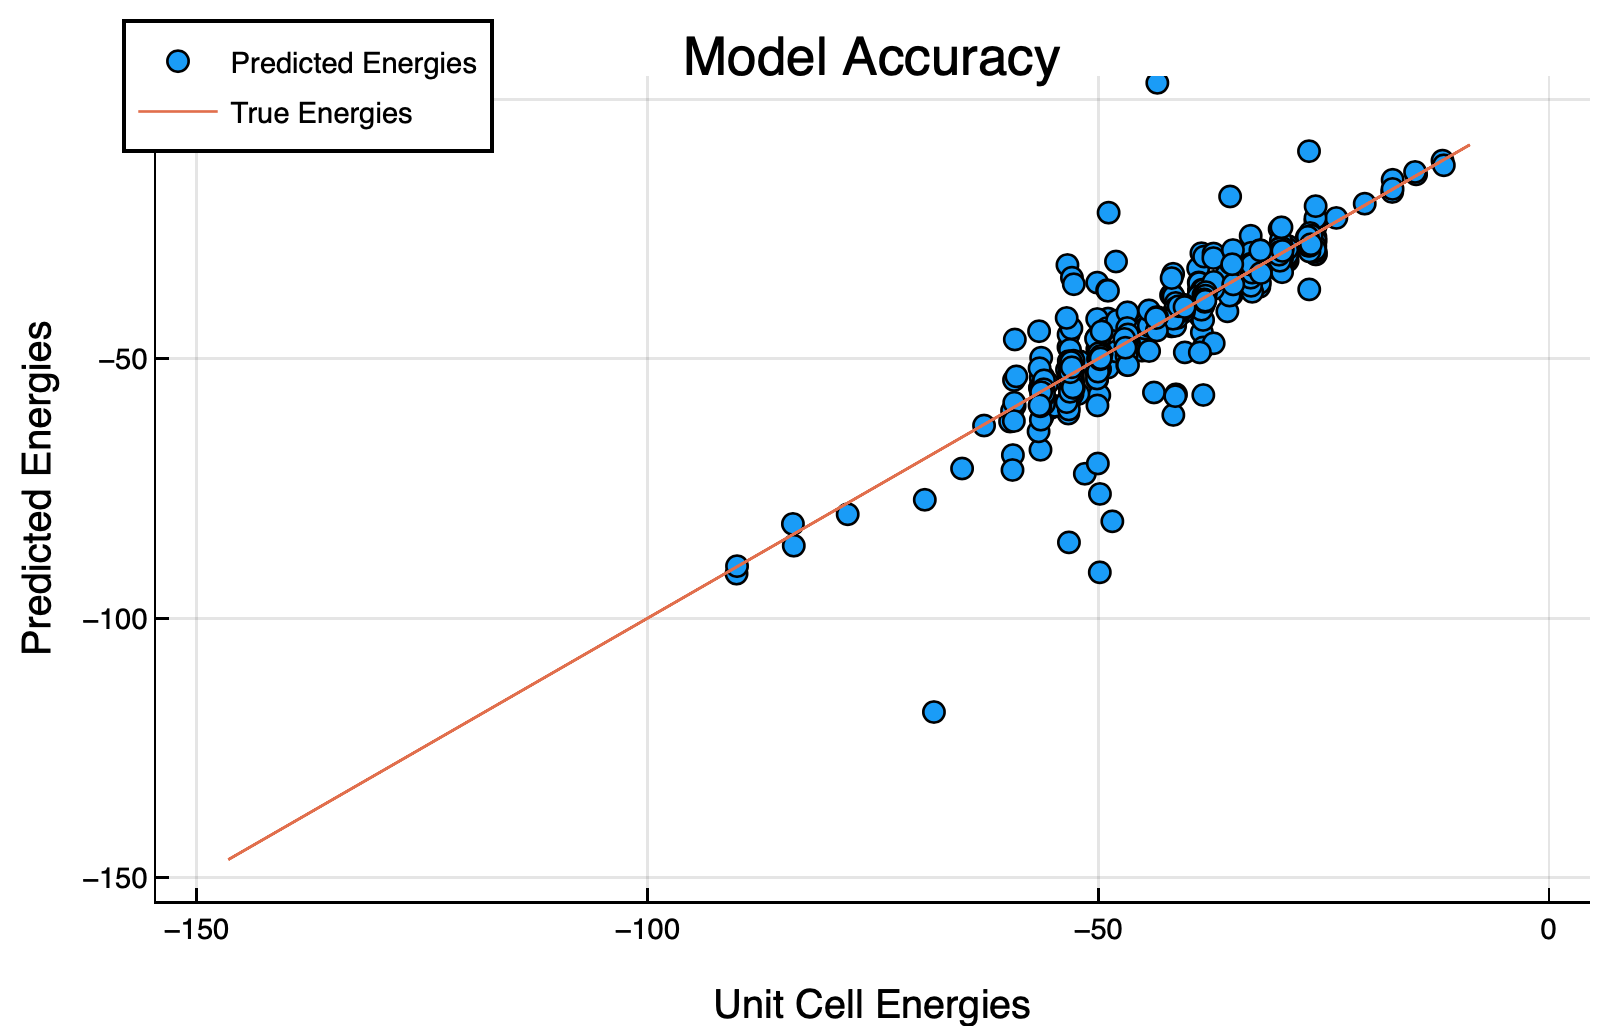
\includegraphics[scale = 0.3]{Figures/accuracyPlot}
\caption{Predicted energies versus the actual energies. The model tested is the same as the one shown in Figure \ref{outputExample}.
\label{accuracyPlot}} 
\end{figure}

\par The method of analysis in Figure \ref{accuracyPlot} works very well for observing one model at a time but interpreting each of the 270 unique models this way would difficult and time consuming. It would be preferable if several data sets could be interpreted at one time.
\par One solution could be a series of heatmaps showing the average error of each model with it's respective parameters. But as discussed above, the average error does not tell the whole story, the number of large errors must also be accounted. Figure \ref{aveErrorHeatmaps} shows five heatmaps, one for each size of training set. The color in each square represents the average error for a specific model. The scale for each subplot is set to be identical to make its analysis easier. A similar cluster of plots can be seen in Figure \ref{numErrorHeatmaps} showing the number of large errors for each model. 

\begin{figure*}
  \begin{subfigure}{0.5\textwidth}
    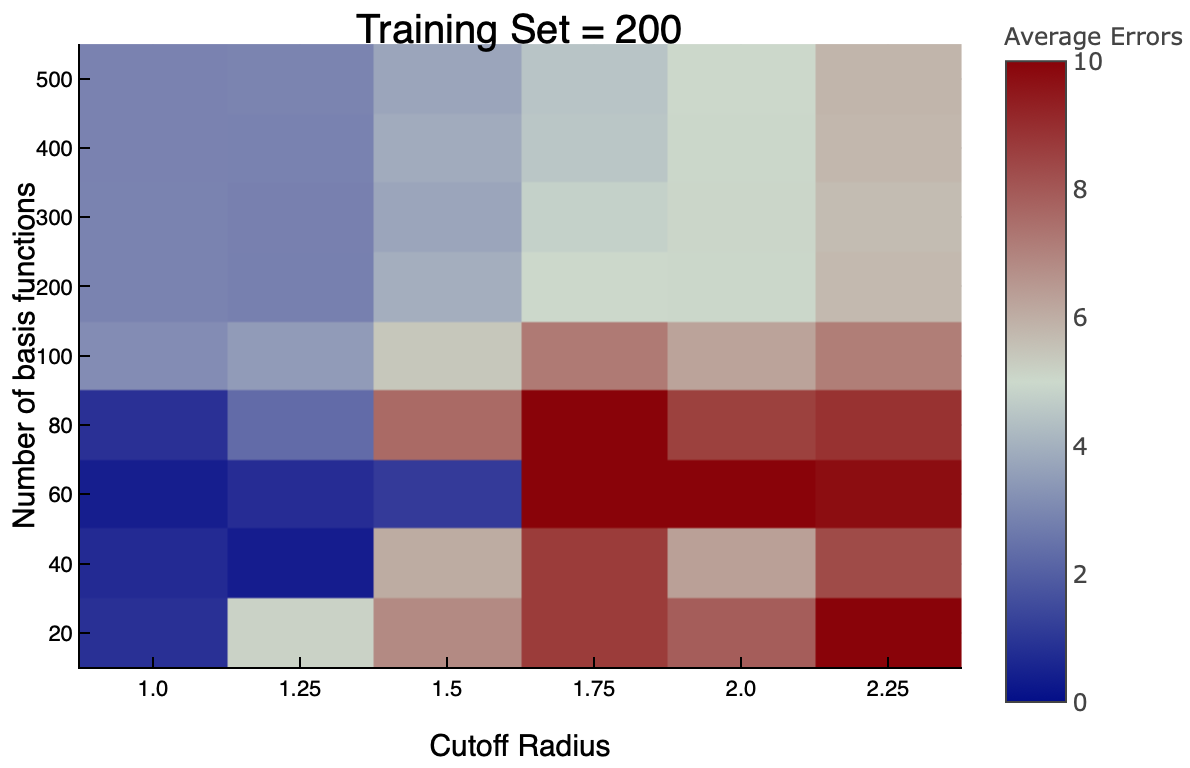
\includegraphics[width=\linewidth]{Figures/aveErrors2}
    \caption{} 
    \label{aveErrors2}
  \end{subfigure}%
  \hspace*{\fill}   % maximize separation between the subfigures
  \begin{subfigure}{0.5\textwidth}
    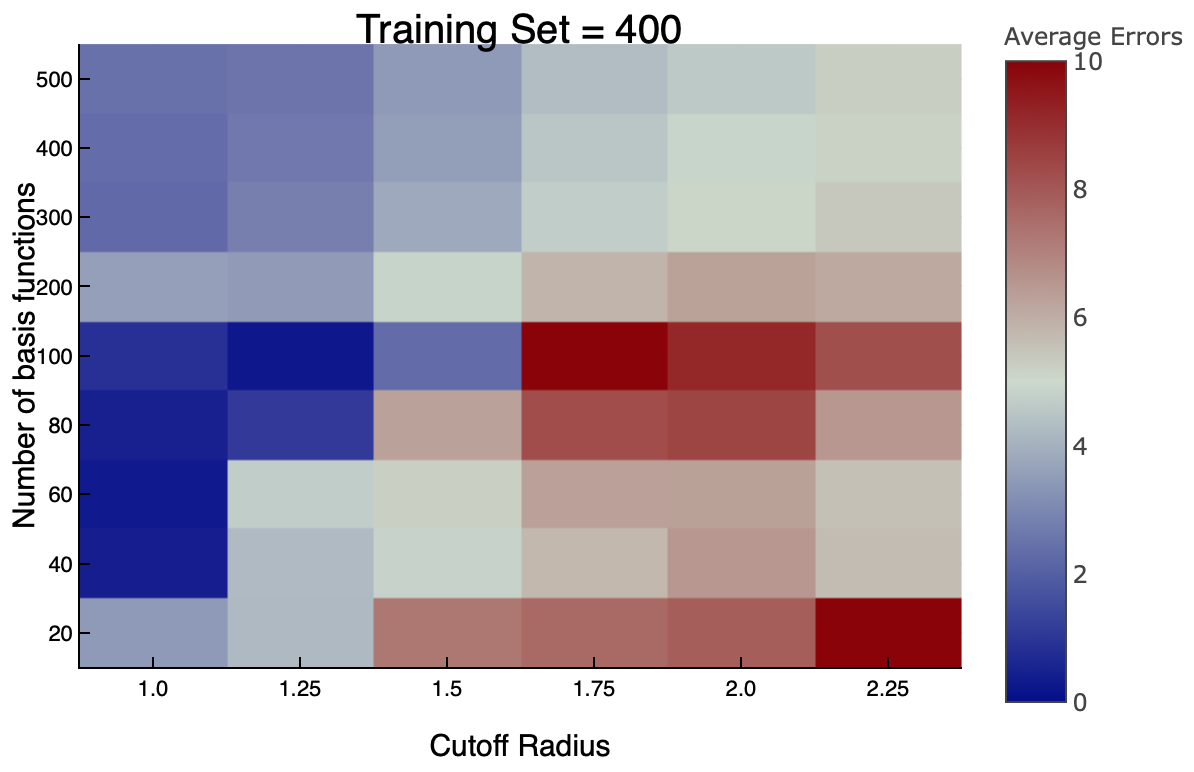
\includegraphics[width=\linewidth]{Figures/aveErrors4}
    \caption{} 
    \label{aveErrors4}
  \end{subfigure}%
    %\hspace*{\fill}   % maximize separation between the subfigures
    \\
  \begin{subfigure}{0.5\textwidth}
    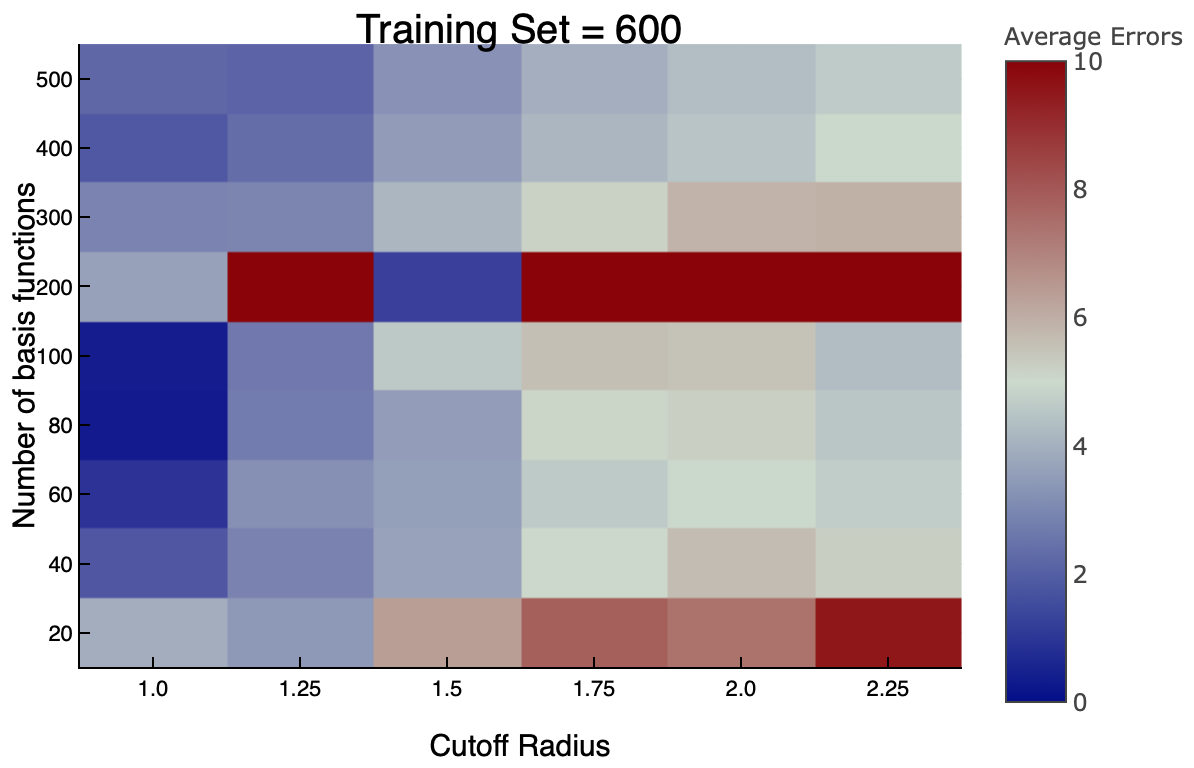
\includegraphics[width=\linewidth]{Figures/aveErrors6}
    \caption{} 
    \label{aveErrors6}
  \end{subfigure}%
    \hspace*{\fill}   % maximize separation between the subfigures
  \begin{subfigure}{0.5\textwidth}
    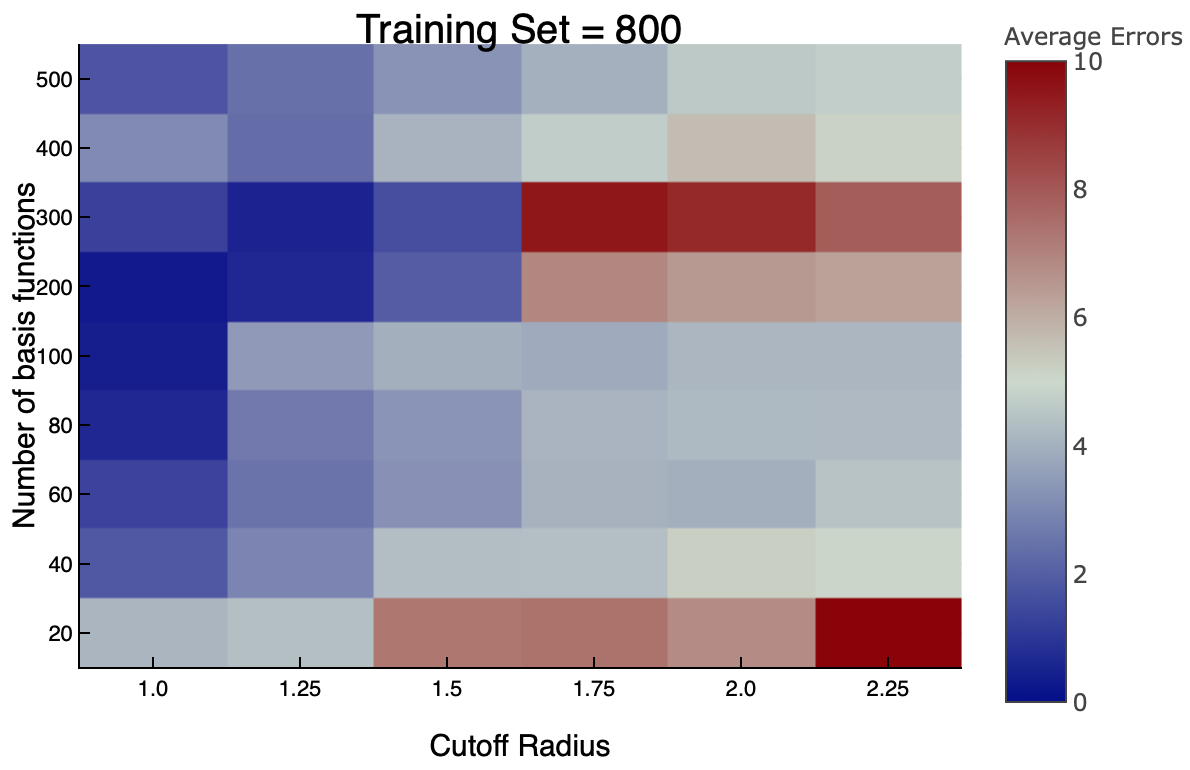
\includegraphics[width=\linewidth]{Figures/aveErrors8}
    \caption{} 
    \label{aveErrors8}
  \end{subfigure}%
    %\hspace*{\fill}   % maximize separation between the subfigures
    \\
  \begin{subfigure}{0.5\textwidth}
    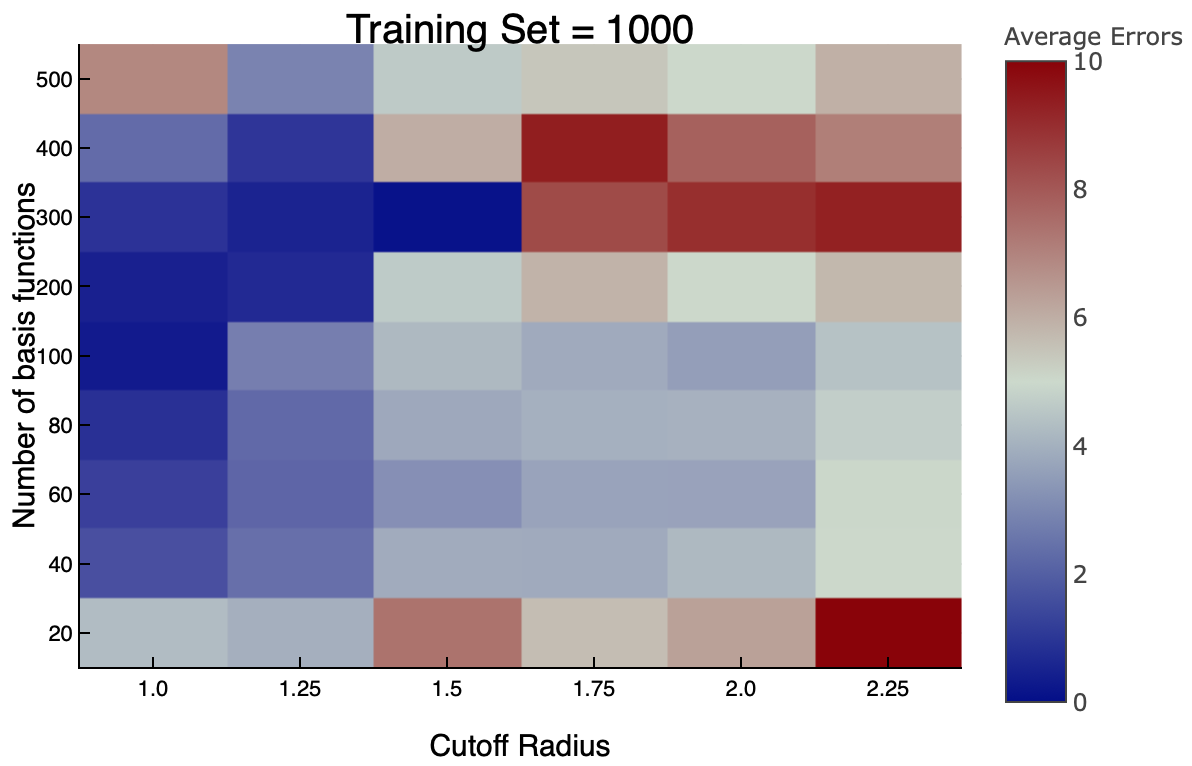
\includegraphics[width=\linewidth]{Figures/aveErrors10}
    \caption{} 
    \label{aveErrors10}
  \end{subfigure}%
\caption{Heatmaps showing the average error of each model produced. The scale for each is fixed from 0eV to 10eV. The effect from removing the large errors from the average can be seen by comparing the more red areas from Figure \ref{numErrorHeatmaps} with the dark blue areas here.}
\label{aveErrorHeatmaps}
\end{figure*}


\begin{figure*}
  \begin{subfigure}{0.5\textwidth}
    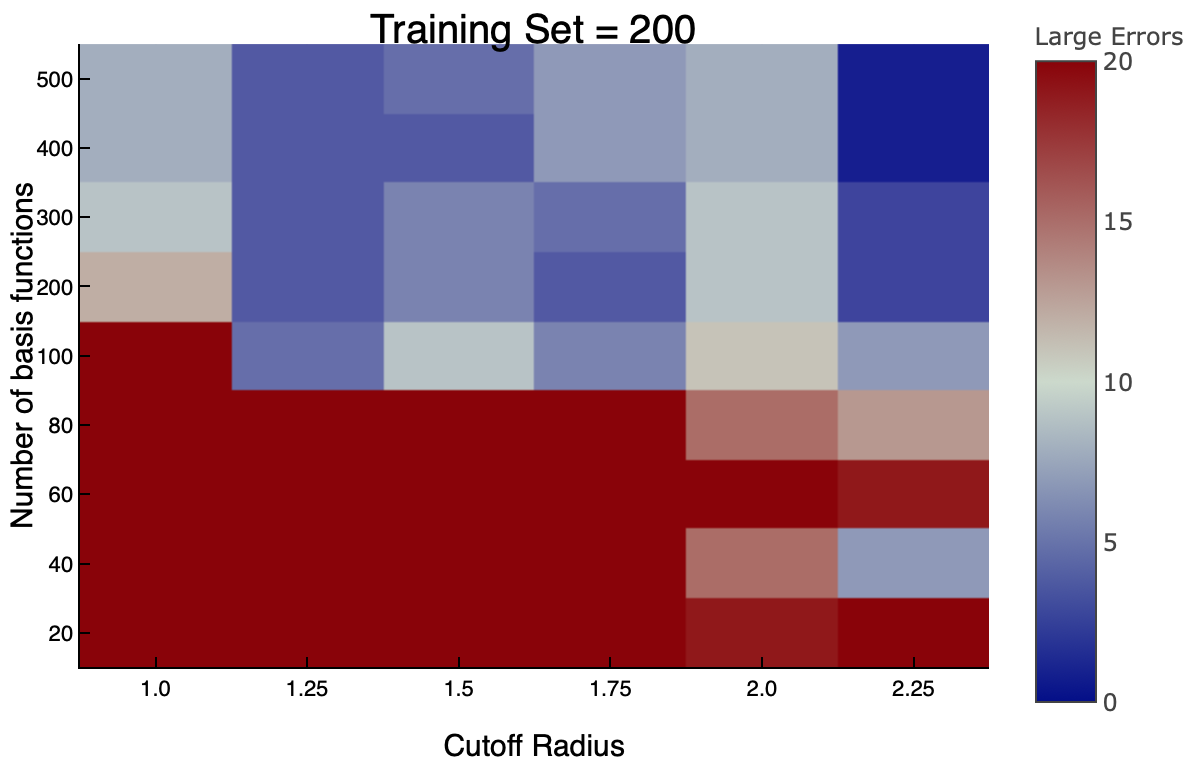
\includegraphics[width=\linewidth]{Figures/numErrors2}
    \caption{} 
    \label{numErrors2}
  \end{subfigure}%
  \hspace*{\fill}   % maximize separation between the subfigures
  \begin{subfigure}{0.5\textwidth}
    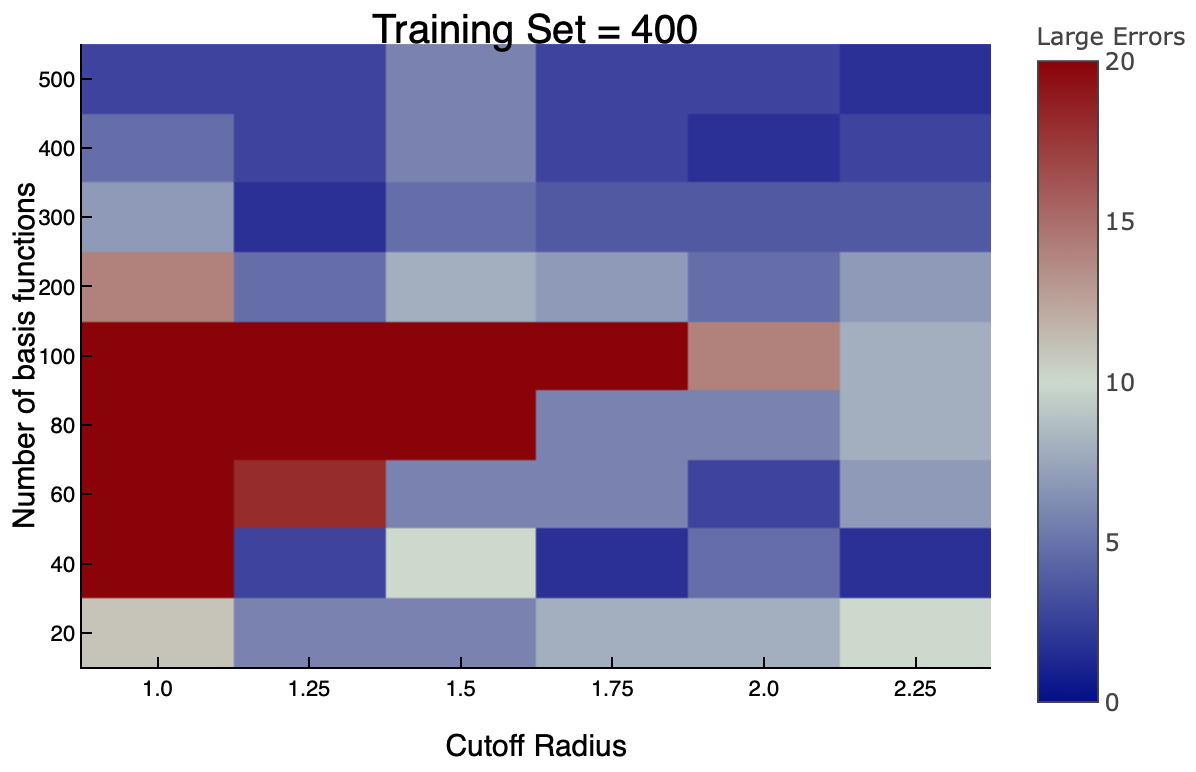
\includegraphics[width=\linewidth]{Figures/numErrors4}
    \caption{} 
    \label{numErrors4}
  \end{subfigure}%
    %\hspace*{\fill}   % maximize separation between the subfigures
    \\
  \begin{subfigure}{0.5\textwidth}
    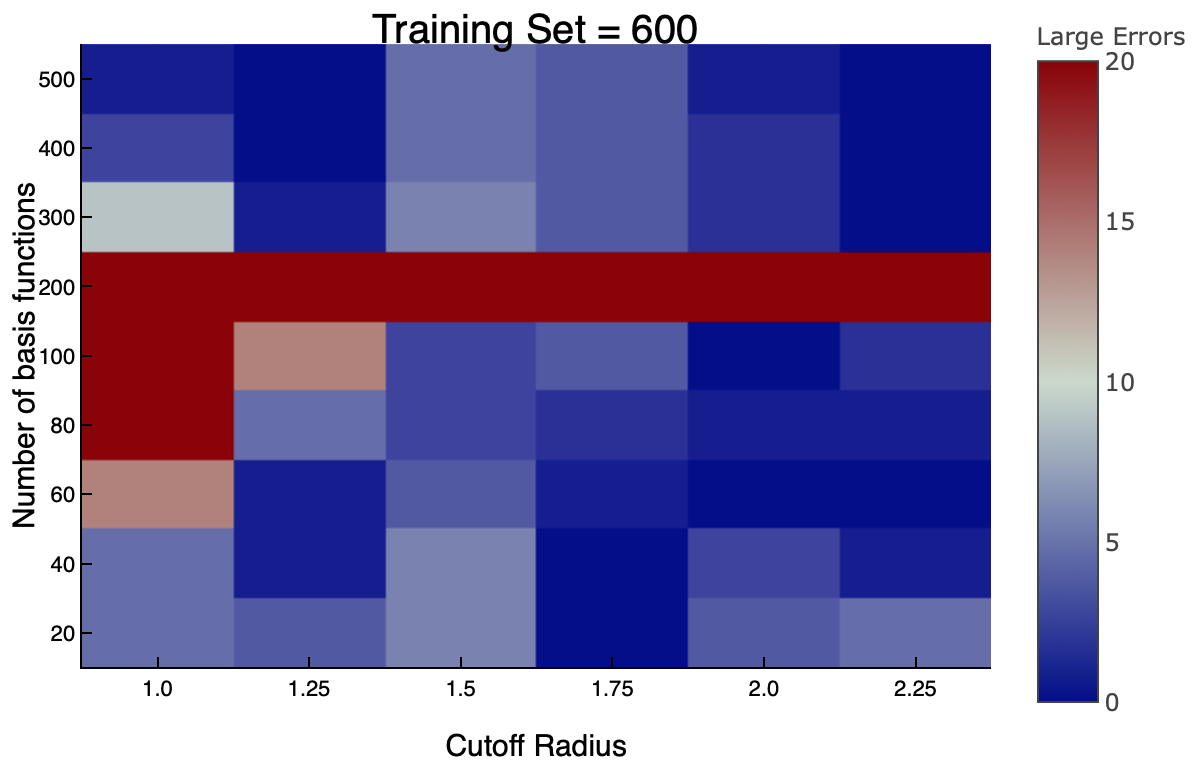
\includegraphics[width=\linewidth]{Figures/numErrors6}
    \caption{} 
    \label{numErrors6}
  \end{subfigure}%
    \hspace*{\fill}   % maximize separation between the subfigures
  \begin{subfigure}{0.5\textwidth}
    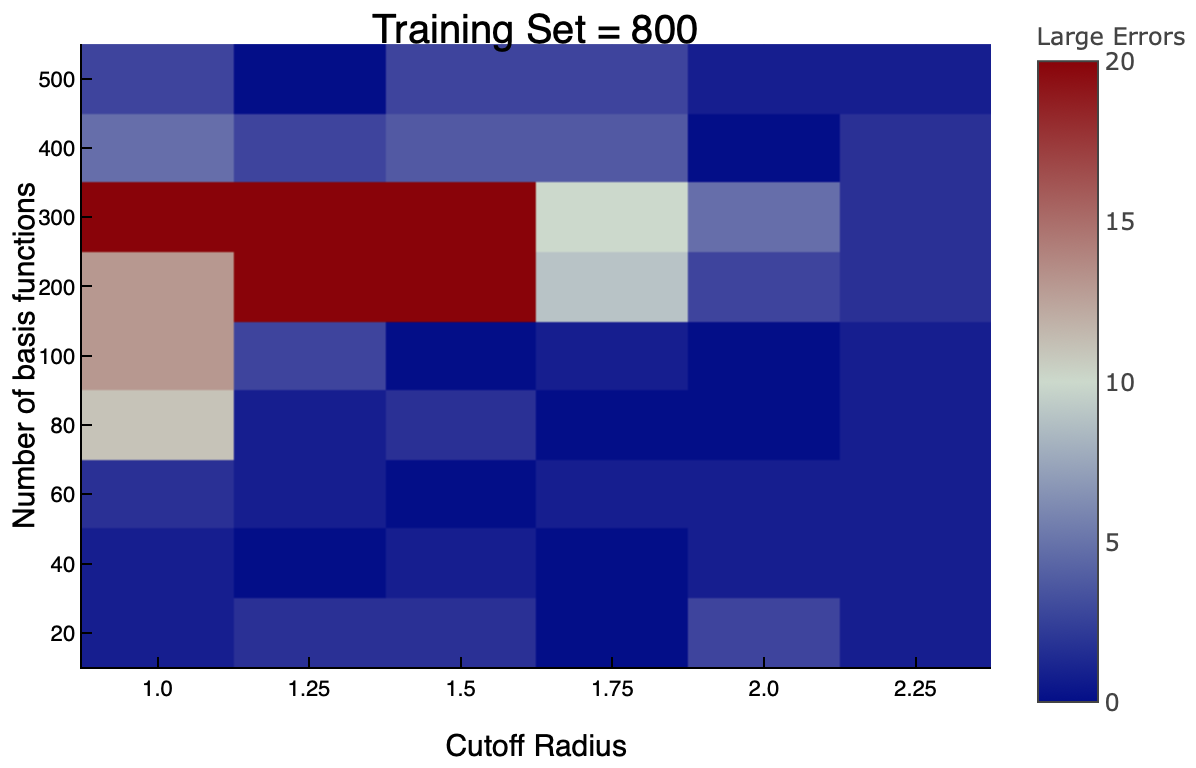
\includegraphics[width=\linewidth]{Figures/numErrors8}
    \caption{} 
    \label{numErrors8}
  \end{subfigure}%
    %\hspace*{\fill}   % maximize separation between the subfigures
    \\
  \begin{subfigure}{0.5\textwidth}
    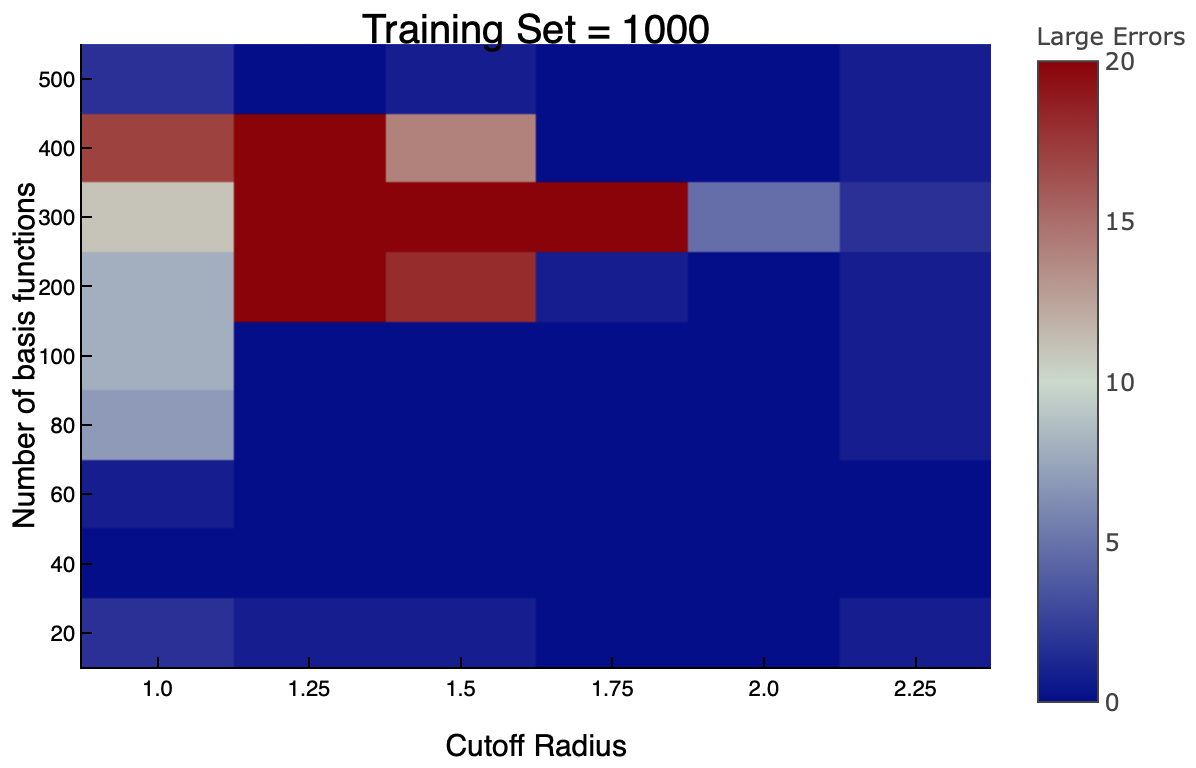
\includegraphics[width=\linewidth]{Figures/numErrors10}
    \caption{} 
    \label{numErrors10}
  \end{subfigure}%
\caption{Heatmaps showing the number of large errors of each model produced. The scale for each is fixed from 0 to 20 errors. Because the scale is fixed, any square with a deep red color has a minimum of 20 errors.}
\label{numErrorHeatmaps}
\end{figure*}


\par The true accuracy and precision of each model can only be realized when comparing its results from Figures \ref{aveErrorHeatmaps} \textit{and} \ref{numErrorHeatmaps}. One without the other does not show the full picture. For example, the lower left corner of Figure \ref{aveErrors2} appears to be surprisingly accurate but when compared to Figure \ref{numErrors2}, it can be seen that these models actually produce a considerable number of large errors. These particular models are not of interest. The models that \textit{are} of interest will be the squares from corresponding subplots in Figures \ref{aveErrorHeatmaps} and \ref{numErrorHeatmaps} that are both blue or blue-ish. It should be noted that one of the reasons the lower left corner of Figure \ref{aveErrors2} is so blue is because the large errors, as seen in Figure \ref{numErrors2}, are all excluded from the overall average error.
\par Figure \ref{numErrors2} includes a large red clump in the bottom right of the plot. This red patch then appears to move upward in each ensuing figure. \ldots \ldots \ldots
\par The most accurate and precise model was trained on 1000 sets, used 40 basis functions, and had an effective radius of 1.0. This model produced 0 large errors and had an average error of only 1.77eV. The second and third best models had very similar input parameters, changing by one step either the size of the training set or the number of basis functions.
\par Why did this model work in some places, but not in others? \ldots \ldots \ldots
\par Because this model was produced using only pair-interactions, implementation of three body interactions has the potential to greatly increase the accuracy of this model. This is, unfortunately, beyond the scope of this research.
\par The success of this simple model may be unique to this silver platinum bond and other particular crystals. But frankly, I have no clue. \ldots\ldots\ldots







\chapter{Conclusion}\label{Sect:conclusion}
\par The models produced were satisfactorily successful. Each provided great insight into which parameters build useful models. Though some models are useful, none are without errors. Using the ``best" model, as mentioned in Section \ref{Sect:results}, new data on silver-platinum crystal configurations can be produced.


\section{Future Work}\label{Sect:futureWork}
\par Using a small set of accurate DFT data, the code written to produce the model in Section \ref{Sect:procedureConstruction} can be easily adapted to construct models for compounds other than Ag-Pt. Such research could be used to determine which compounds can be accurately predicted using a simple pair-interaction model. A successful model can quickly predict formation energies for a variety of crystal configurations. These formation energies could then be used to construct the material’s phase diagram and determine which phases are thermodynamically stable.
\par Because the models produced in this paper used only pair-interactions, their effectiveness is limited by their simplicity. Implementation of three-body interactions has the potential to greatly increase the accuracy of these models.
\par Citations yet to be included: \cite{_AFLOW} \cite{Kohn1965} \cite{curt2005scienceandtech} \cite{curtarolo2003predicting} \cite{Kresse:1999wc} \cite{kresse1993abinitio} \cite{Blochl:1994dx} \cite{kresse1996efficiency} \cite{monkhorst1976special} \cite{sanchez1984generalized} \cite{laks1992efficient} \cite{lerch2009uncle} \cite{cockayne2010building} \cite{nelson2013compressive}


%\bibliographystyle{apj}
%\bibliographystyle{ieeetr}
\bibliography{refs}

%\section{Bibliography}
%\begin{itemize}
%\item Lennard-Jones potential info?
%\item Solid State book
%\item ?
%\end{itemize}



\end{document}



